\documentclass[10pt]{article}
\usepackage{commands}
%\renewcommand{\familydefault}{\sfdefault}
\usepackage[sc]{mathpazo}
\usepackage{siunitx}
%\usepackage{tgpagella}
\numberwithin{equation}{section}

\begin{document}
\begin{tcolorbox}
  \begin{center}
  \begin{Large}
    \textbf{Ryden Solutions} \\
    \vspace{5pt}
  \end{Large}
  \begin{large}
        Rio Weil \\
\vspace{5pt}
    \emph{This document was typeset on \today}
  \end{large}
  \end{center}
\end{tcolorbox}

\begin{center}
  Solutions to problems from Ryden's ``Introduction to Cosmology'', 2nd ed.

\end{center}
\addtocontents{toc}{\protect\hypertarget{toc}{}}
\tableofcontents

\newpage
\section[Introduction]{\hyperlink{toc}{Introduction}}
\section[Fundamental Observations]{\hyperlink{toc}{Fundamental Observations}}
\subsection{Human blackbody radiation}
The energy density of blackbody radiation is given by:
\begin{equation}
  \e_\gamma = \alpha T^4
\end{equation}
Approximating a human being as a sphere with volume 1\si{m^3}, an considering that photons travel at speed $c$ we have that the rate of energy radiation is:
\begin{equation}
  \boxed{E = c A \e_\gamma = cA\alpha T^4 \sim 2.10 \times 10^3 \si{W}}
\end{equation} 

\subsection{CMB photon rate}
We can calculate the photon number density of the CMB to be:
\begin{equation}
  n_\gamma = \beta T^3 = (2.029 \times 10^{7}\si{m^{-3}.K^{-3}})(2.8255\si{K})^3 = 4.107 \times 10^8 \si{m^{-3}}
\end{equation}
Approximating our body to be a perfect sphere with cross sectional area $A \sim 1\si{m}$, since photons travel at a rate $c \si{m.s^{-1}}$ the rate at which they pass through us is:
\begin{equation}
  \boxed{r \sim c A n_\gamma = (3.00 \times 10\si{m.s^{-1}})(1\si{m^2})(4.107 \times 10^8 \si{m^{-3}}) = 1.23 \times 10^{17} \si{s^{-1}}}
\end{equation}

\subsection{How long for the CMB to warm you up?}
The energy per photon of the CMB is:
\begin{equation}
  \frac{\e_\gamma}{n_\gamma} = 1.02 \times 10^{-22}\si{J}
\end{equation}
The energy required to raise my temperature by $1\si{nK}$ is:
\begin{equation}
  \Delta E = Cm\Delta T = (4200\si{J.kg^{-1}.K^{-1}})(50\si{kg})(10^{-9}\si{K}) = 2.1 \times 10^{-4}\si{J}
\end{equation}
So solving for the time to heat up by 1 nanoKelvin:
\begin{equation}
  \boxed{t_{1\si{nK}} = \frac{\Delta E}{r\frac{\e_\gamma}{n_\gamma}} \sim 16.8\si{s}}
\end{equation}


\subsection{Tired Light}
We start with the energy loss per unit distance propsed by the ``tired light hypothesis'':
\begin{equation}
    \dod{E}{r} = -kE
\end{equation}
This is the all-too-famous exponential decay ODE, which has solution:
\begin{equation}
    E(r) = C\exp(-kr)
\end{equation}
In principle we could use separation of variables to solve the ODE, but let's just verify that this is the correct solution:
\begin{equation}
    \dod{}{r}\left(C\exp(-kr)\right) = -kC\exp(-kr) = -kE\quad  \checkmark
\end{equation}
Letting $E(0) = E_0$ be the distance of the energy of the photon when emitted (before it has travelled and lost energy), we get:
\begin{equation}
    E_0 = E(0) = C\exp(-k(0)) = C \implies C = E_0
\end{equation}
Therefore:
\begin{equation}\label{expsol}
    E(r) = E_0\exp(-kr)
\end{equation}
Now, using the energy-momentum relation and the DeBroglie wavelength relation, we have:
\begin{equation}
    E = pc = \frac{hc}{\lambda}
\end{equation}
So substituting this into \eqref{expsol} we get:
\begin{equation}
    \frac{hc}{\lambda_r} = \frac{hc}{\lambda_0}\exp(-kr)
\end{equation}
Where $\lambda_r$ is the observed/measured photon wavelength at distance $r$ from the source and $\lambda_0$ is the photon wavelength measured at the source. Rearranging we obtain:
\begin{equation}\label{lambdas}
    \frac{\lambda_r}{\lambda_0} = \exp(kr)
\end{equation}
Now we recall the definition of redshift:
\begin{equation}
    z = \frac{\lambda_r - \lambda_0}{\lambda_0} = \frac{\lambda_r}{\lambda_0} - 1
\end{equation}
Substituting this into \eqref{lambdas} we get:
\begin{equation}
    z = \exp(kr) - 1
\end{equation}
Which adding one and taking the logarithm of both sides we get:
\begin{equation}
    \log(1 + z) = kr
\end{equation}
If $z \ll 1$, then by Taylor expanding to first order we obtain:
\begin{equation}
    \log(1+z) \approx z
\end{equation}
So in this limit we have:
\begin{equation}\label{ansq1}
    \boxed{z = kr}
\end{equation}
From which we see a linear distance-redshift relation. For the last part of the question, we recall Hubble's Law:
\begin{equation}
    z = \frac{H_0}{c}r
\end{equation}
So comparing this with \eqref{ansq1}, the value of $k$ to yield a Hubble constant of $H_0 = 68 \si{km.s^{-1}.Mpc^{-1}}$ must be:
\begin{equation}
    \boxed{k = \frac{H_0}{c} = 2.3 \times 10^{-4}\si{Mpc^{-1}}}
\end{equation}

\subsection{CMB Cutoff - The Cosmic Infrared background}
We start with the number density for CMB photons:
\begin{equation}
  n(f)df = \frac{\e(f)df}{hf} = \frac{8\pi}{c^3}\frac{f^2df}{\exp(hf/kT) - 1}
\end{equation}
Since $hf > E_0 \gg kT$, we have that $\exp(hf/kT) \gg 1$ and so $\exp(hf/kT) -1 \sim \exp(hf/kT)$. This yields:
\begin{equation}
  n(f)df \approx \frac{8\pi}{c^3}f^2\exp(-\frac{hf}{kT})df
\end{equation}
Now, to get $n(hf > E_0)$ we integrate this expression from $E_0/h$ to $\infty$.
\begin{equation}
  n(hf > E_0) = \int_{E_0/h}^\infty \frac{8\pi}{c^3}f^2\exp(-\frac{hf}{kT})df
\end{equation}
Integrating by parts (with $u = f^2, dv = \exp(-hf/kT)$), we have:
\begin{equation}
  n(hf > E_0) = \frac{8\pi}{c^3}\left(\left.f^2\frac{-kT}{h}\exp(-\frac{hf}{kT})\right|_{E_0/h}^\infty - \int_{E_0/h}^\infty 2f\frac{-kT}{h}\exp(-\frac{hf}{kT})df\right)
\end{equation}
The term at infinity goes to zero, so:
\begin{equation}
  n(hf > E_0) = \frac{8\pi}{c^3}\left(\frac{kTE_0^2}{h^3}\exp(-\frac{E_0}{kT})+ \frac{2kT}{h}\int_{E_0/h}^\infty f\exp(-\frac{hf}{kT})df\right)
\end{equation}
We now integrate by parts again (with $u = f, dv = \exp(-\frac{hf}{kT})$) to get:
\begin{equation}
  n(hf > E_0) = \frac{8\pi}{c^3}\left(\frac{kTE_0^2}{h^3}\exp(-\frac{E_0}{kT})+ \frac{2kT}{h}\left(\left.f\frac{-kT}{h}\exp(-\frac{hf}{kT})\right|_{E_0/h}^\infty - \int_{E_0/h}^\infty \frac{-kT}{h}\exp(-\frac{hf}{kT})df\right)\right)
\end{equation}
Again the term at infinity goes to zero and we get:
\begin{equation}
  n(hf > E_0) = \frac{8\pi}{c^3}\left(\frac{kTE_0^2}{h^3}\exp(-\frac{E_0}{kT})+ \frac{2kT}{h}\left(\frac{kTE_0}{h^2}\exp(-\frac{E_0}{kT}) + \frac{kT}{h}\int_{E_0/h}^\infty\exp(-\frac{hf}{kT})df\right)\right)
\end{equation}
Finally the last integral is easy:
\begin{equation}
  n(hf > E_0) = \frac{8\pi}{c^3}\left(\frac{kTE_0^2}{h^3}\exp(-\frac{E_0}{kT})+ \frac{2kT}{h}\left(\frac{kTE_0}{h^2}\exp(-\frac{E_0}{kT}) + \frac{kT}{h}\left(\left.\frac{-kT}{h}\exp(-\frac{hf}{kT})\right|_{E_0/h}^\infty\right)\right)\right)
\end{equation}
So after this tedious calculation, we have:
\begin{equation}
  n(hf > E_0) = \frac{8\pi}{c^3}\exp(-\frac{E_0}{kT})\left[\frac{kTE_0^2}{h^3} + \frac{2k^2T^2E_0}{h^3} + \frac{2k^3T^3}{h^3}\right]
\end{equation}
Using that $E_0 \gg kT$ again, we can neglect all but the first term (so we could have really avoided the latter two integration steps, but alas):
\begin{equation}
  n(hf > E_0) \approx \frac{8\pi kTE_0^2}{c^3h^3}\exp(-\frac{E_0}{kT})
\end{equation}
Now taking the ratio of this with $n_\gamma$:
\begin{equation}
  \boxed{\frac{n(hf > E_0)}{n_\gamma} \approx \frac{\frac{8\pi kTE_0^2}{c^3h^3}\exp(-\frac{E_0}{kT})}{\frac{2.4041}{\pi^2}\frac{k^3}{\hbar^3c^3}T^3} = 0.42\left(\frac{E_0}{kT}\right)^2\exp(-\frac{E_0}{kT})}
\end{equation}
which was the desired formula. Next, we calculate the fraction of ``CMB'' photons that are actually far-IR photons. We first consider the wavelength-frequency relation for light:
\begin{equation}
  c = \lambda f
\end{equation}
so $\lambda < 1\si{mm}$ corresponds to $f > 3 \times 10^{11}\si{Hz}$ and so:
\begin{equation}
  E = hf > 2 \times 10^{-22}\si{J}
\end{equation}
So using the above derived relation with $T = 2.7255\si{K}$ we have:
\begin{equation}
  \boxed{\frac{n(hf > 2 \times 10^{-22}\si{J})}{n_\gamma} \approx 0.42\left(\frac{2 \times 10^{-22}\si{J}}{k\cdot 2.7255\si{K}}\right)^2\exp(-\frac{2 \times 10^{-22}\si{J}}{k\cdot 2.7255\si{K}}) = 0.058}
\end{equation}


\subsection{CMB Cutoff - The Other Direction}
We again recall the number density of the CMB photons:
\begin{equation}
  n(f)df = \frac{8\pi}{c^3}\frac{f^2df}{\exp(hf/kT) - 1}
\end{equation}
Since $kT \gg E_0 > hf$, we have that:
\begin{equation}
  \exp(\frac{hf}{kT}) \approx 1 + \frac{hf}{kT}
\end{equation}
by Taylor expanding to first order. The number density in this regime therefore becomes:
\begin{equation}
  n(f)df \approx \frac{8\pi}{c^3}\frac{f^2df}{1 + \frac{hf}{kT} - 1} = \frac{8\pi k T}{hc^3}fdf
\end{equation}
Integrating this from $0$ to $E_0/h$, we obtain $n(hf < E_0)$:
\begin{equation}
  n(hf < E_0) \approx \int_{0}^{E_0/h}\frac{8\pi k T}{hc^3}fdf = \frac{4\pi kT}{hc^3}\left. f^2\right|_0^{E_0/h} = \frac{4\pi kTE_0^2}{h^3c^3}
\end{equation}
So solving for the fraction of photons in the CMB with $hf < E_0$ we have:
\begin{equation}
  \boxed{\frac{n(hf < E_0)}{n_\gamma} \approx \frac{\frac{4\pi kTE_0^2}{h^3c^3}}{\frac{2.4041}{\pi^2}\frac{k^3}{\hbar^3c^3}T^3} = 0.21\left(\frac{E_0}{kT}\right)^2}
\end{equation}
Solving for the fraction of CMB photons with $\lambda > 3\si{cm}$ (and hence capable of passing through the Earth's atmosphere) we again use the wavelength-frequency relation for light of $c = \lambda f$. $\lambda > 3\si{cm}$ corresponds to $f < 10^{10}\si{Hz}$ so:
\begin{equation}
  E = hf < 6.63 \times 10^{-24}\si{J}
\end{equation}
So using our obtained relation with $T = 2.7255\si{K}$ we have:
\begin{equation}
  \boxed{\frac{n(hf < 7 \times 10^{-24}\si{J})}{n_\gamma} \approx  0.21\left(\frac{7 \times 10^{-24}\si{J}}{k\cdot 2.7255\si{K}}\right)^2 = 0.0065}
\end{equation}
\newpage 
\section[Newton versus Einstein]{\hyperlink{toc}{Newton versus Einstein}}

\subsection{Evidence for electrical neutrality}
Through astronomical observations, we notice that gravitational forces dominate dynamics in the universe on large scales. However, electrostatic forces are much stronger than gravitational. A simple demonstration of this is given by comparing the magnitudes of the gravitational and electrostatic forces between an electron and proton. At a distance $r$, the gravitational force between an electron and proton (in the Newtonian picture) is given by:
\begin{equation}
    \abs{F_g} = \frac{Gm_p m_e}{r^2} = \frac{1}{r^2}(6.67 \times 10^{-11} \si{N.kg^{-2}.m^2})(1.67 \times 10^{-27} \si{kg})(9.11 \times 10^{-31}\si{kg}) = \frac{1.01 \times 10^{-66}}{r^2} \si{N}
\end{equation}
And the elecctrostatic force is given by:
\begin{equation}
    \abs{F_e} = \frac{k e^2}{r^2} = \frac{1}{r^2}(8.99 \times 10^{9} \si{N.C^{-2}.m^2})(1.60 \times 10^{-19} C)^2 = \frac{2.30\times 10^{-28}}{r^2} \si{N}
\end{equation}
Taking the ratio we have:
\begin{equation}
    \abs{\frac{F_e}{F_g}} = \abs{\frac{\frac{2.30\times 10^{-28}}{r^2} \si{N}}{\frac{1.01 \times 10^{-66}}{r^2} \si{N}}} = 2.28 \times 10^{38}
\end{equation}
As we can see from this example, electrostatic forces are much stronger than gravitational (38 orders of magnitude stronger in this case!). Hence if there was a large charge imbalance in the universe, we would observe that electrostatic forces would dominate large-scale dynamics rather than gravitational. This however disagrees with our observations, and we conclude that the universe must be (mostly) electrically neutral.

\subsection{Angular Width on a sphere}
We recall that the metric for a sphere of radius $R$ is given by:
\begin{equation}
    dl^2 = dr^2 + R^2\sin^2\left(\frac{r}{R}\right)d\theta^2
\end{equation}
So we can write the width $dl$ of the object using the above equation. Since $dl \ll R$, we can take the entire width of the object to be located at the same distance $r$ away from us (the observer). In other words, in this limit we have $dr = 0$ and hence the above reduces to:
\begin{equation}
    dl^2 = R^2\sin^2\left(\frac{r}{R}\right)d\theta^2
\end{equation}
Isolating for the angular width of the object, we obtain:
\begin{equation}
    \boxed{d\theta = \frac{dl}{R\sin(\frac{r}{R})}}
\end{equation}
As we take $r \to \pi R$ (i.e. the object is located at the antipode) we have:
\begin{equation}
   \lim_{r \to R\pi} d\theta = \lim_{r \to R\pi} \frac{dl}{R\sin(\frac{r}{R})} = \infty
\end{equation}
as the denominator goes to 0 ($\lim_{r \to R\pi}\sin(\frac{r}{R}) = \sin(\frac{R\pi}{R}) = \sin(\pi) = 0$). The angular width is minimized when the object lies on the equator, where $r = \frac{R\pi}{2}$ and $d\theta = \frac{dl}{R}$, and this angular width increases to infinity as the object approaches the antipode of the sphere. For an object at the antipode, all lines of sight from the observer lead to the object, and it therefore fills the horizon.

\subsection{The Earth isn't flat!}
We choose our coordinate system such that the origin is located in the center of the sphere, and we as the oberver are located at the north pole. The circle drawn on the sphere is at a fixed distance $r$ from us on the north pole, and therefore each point on the sphere is at a fixed polar angle $\theta$. The radius of this circle as measured as an outside observer (not located on the sphere) is $R \sin\theta$.
\begin{figure}[htbp]
    \centering
    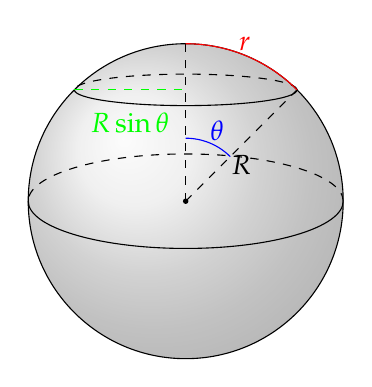
\begin{tikzpicture}
        \shade[ball color = gray!40, opacity = 0.4] (0,0) circle (2cm);
        \draw (0,0) circle (2cm);
        \draw (-2,0) arc (180:360:2 and 0.6);
        \draw[dashed] (2,0) arc (0:180:2 and 0.6);
        \fill[fill=black] (0,0) circle (1pt);
        \draw[dashed] (0,0) -- node[below]{$R$} (1.414,1.414);
        \draw (-1.414, 1.414) arc (180:360:1.414 and 0.2);
        \draw[dashed] (1.414, 1.414) arc (0:180:1.414 and 0.2);
        \draw[dashed] (0, 0) -- (0, 2);
        \draw[blue] (0, 0.8) arc (90:45:0.8);
        \node[blue] at (0.4, 0.9) {$\theta$};
        \draw[red] (0, 2) arc (90:45:2);
        \node[red] at (0.75, 2) {$r$};
        \draw[dashed, green] (-1.414, 1.414) -- (0, 1.414);
        \node[green] at (-0.707, 1) {$R\sin\theta$};
    \end{tikzpicture}
    \caption{Illustration of setup of Problem 3.3}
    \label{fig3.3}
\end{figure}
The circumference of the circle is therefore given by:
\begin{equation}
    C = 2\pi R \sin \theta
\end{equation}
Now, we recall that the arclength $r$ is related to the polar angle and sphere radius by:
\begin{equation}
    r = R\theta.
\end{equation}
So substituing this into the circumference, we obtain:
\begin{equation}\label{circsphere}
    \boxed{C = 2\pi R\sin(\frac{r}{R})}
\end{equation}
which was the claimed formula. For the second part of the question, we consider that for a flat space, the circumference would be measured to be:
\begin{equation}
    C_f = 2\pi r.
\end{equation}
In the limit $r \ll R$, we can Taylor expand the circumference as given in Eq. \eqref{circsphere} to obtain that:
\begin{equation}
    C_s \approx 2\pi R\left(\frac{r}{R} - \frac{r^3}{6R^3}\right) = 2\pi r - \frac{\pi r^3}{3R^2}
\end{equation}
Hence the difference between the circumference measured in Euclidean space versus a sphere would be given by:
\begin{equation}
    \abs{C_f - C_s} \approx \abs{2\pi r - (2\pi r - \frac{\pi r^3}{3R^2})} = \frac{\pi r^3}{3R^2}.
\end{equation}
We can measure distances within an error of $\pm 1\si{m}$, so to convince ourselves that Earth is spherical rather than flat, we require that the circumference differnece be:
\begin{equation}
    \abs{C_f - C_s} > 1\si{m}
\end{equation}
So approximately:
\begin{equation}
    \frac{\pi r^3}{3R^2} > 1 \si{m}
\end{equation}
Rearranging, we have:
\begin{equation}
    r > \sqrt[3]{\frac{3\si{m} R^2}{\pi}}
\end{equation}
And substituing $R = 6400\si{km}$ we get:
\begin{equation}
    \boxed{r > 34\si{km}}
\end{equation}

\subsection{Area Bounds for Equilateral Triangles}
\textbf{Case 1: $\kappa = +1$}. No, we cannot draw an equilateral triangle of arbitrarily large surface area $A$ in this case. A simple counterargument is that a sphere has surface area $4\pi R^2$, so immediately no triangle with area larger than that is possible. For a calculation of the maximum area of a triangle, we require a thoughtful argument. First, recall the equation for the sum of three angles of a triangle of area $A$ on a surface of a sphere of radius $R$:
\begin{equation}
    \alpha + \beta + \gamma  = \pi + \frac{A}{R^2}
\end{equation}
For an equiliateral triangle, $\alpha = \beta = \gamma$, so:
\begin{equation}\label{sphereangles}
    3\alpha = \pi + \frac{A}{R^2}
\end{equation}
WLOG, we can choose our coordinate system that the first point of the triangle is on the north pole, the second point is a distance $r$ from the north pole on the sphere with azimuthal angle $\phi = 0$, and the third point is also a distance $r$ from the north pole on the sphere with azimuthal angle $\phi = \alpha$.

\begin{figure}[htbp]
    \centering
    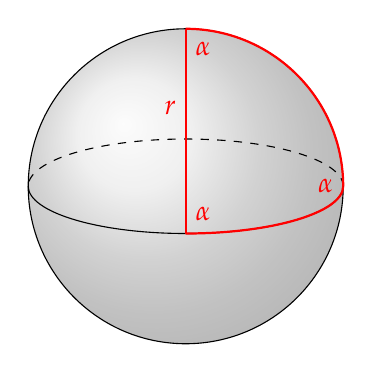
\begin{tikzpicture}
        \shade[ball color = gray!40, opacity = 0.4] (0,0) circle (2cm);
        \draw (0,0) circle (2cm);
        \draw (-2,0) arc (180:360:2 and 0.6);
        \draw[dashed] (2,0) arc (0:180:2 and 0.6);
        \draw[red, thick] (0, 2) arc (90:0:2);
        \draw[red, thick] (0, 2) -- (0, -0.6);
        \draw[red, thick] (0,-0.6) arc (270:360:2 and 0.6);
        \node[red, left] at (0, 1) {$r$};
        \node[red, right] at (0, 1.75) {$\alpha$};
        \node[red, right] at (0, -0.35) {$\alpha$};
        \node[red, left] at (2, 0) {$\alpha$};
    \end{tikzpicture}
    \caption{Illustration of the triangle drawn for the spherical case of Problem 3.4.}
    \label{fig3.4}
\end{figure}

\noindent We now recall the area element on the sphere is given as:
\begin{equation}
    dA = R d\theta \cdot R \sin\theta d\phi = R^2 d\theta d\phi 
\end{equation}
Where $Rd\theta$ is the polar distance and $R\sin\theta d\phi$ is the azimuthal distance. With the setup as described, the area of the triangle may be calculated via integration. We integrate from $0 \leq \theta \leq \frac{r}{R}$ (recalling that $r = R\theta$) and from $0 \leq \phi \leq \alpha$:
\begin{equation}
    A = \iint_{\text{triangle}} dA = R^2 \int_{0}^{r/R} \sin\theta d\theta \int_{0}^{\alpha} d\phi 
\end{equation}
Carrying out these two easy integrals, we obtain:
\begin{equation}
    A = R^2 \left(1 - \cos(\frac{r}{R})\right)\alpha
\end{equation}
Isolating for $\alpha$, we obtain:
\begin{equation}
    \alpha = \frac{A}{R^2\left(1 - \cos(\frac{r}{R})\right)}
\end{equation}
Plugging this into \eqref{sphereangles}, we get:
\begin{equation}
    3\frac{A}{R^2\left(1 - \cos(\frac{r}{R})\right)} = \pi + \frac{A}{R^2}
\end{equation}
Isolating for $A$ we have:
\begin{equation}
    A = \pi R^2 \frac{1 - \cos(\frac{r}{R})}{2 + \cos(\frac{r}{R}) }
\end{equation}
The largest that $r$ can possibly be is when $r = \pi R$ (the base of the triangle lies on the south pole), and so:
\begin{equation}
    \boxed{A_{\text{max}} = \pi R^2 \frac{1 - \cos(\frac{\pi R}{R})}{2 + \cos(\frac{\pi R}{R}) } = \pi R^2 \frac{1 - (-1)}{2 - 1} = 2\pi R^2}
\end{equation}
In other words, the largest an equilateral triangle can be in this case is being half of the sphere!

\noindent \textbf{Case 2: $\kappa = 0$}. We can draw an equilateral triangle of arbitrarily large surface area $A$ in this case. On a flat plane, there is no upper bound to how large you want to draw your shapes!

\noindent \textbf{Case 3: $\kappa = -1$}. No, we cannot draw an equilateral triangle of arbitrarily large surface area $A$ in this case. Consider the equation that gives the sum of three angles of a triangle on a 2-D surface of uniform negative curvature (with radius of curvature $R$):
\begin{equation}
    \alpha + \beta + \gamma = \pi - \frac{A}{R^2}
\end{equation}
For an equilateral triangle, $\alpha = \beta = \gamma$ so:
\begin{equation}
    3\alpha = \pi - \frac{A}{R^2}
\end{equation}
$\alpha$ cannot be negative if we are to have a physical shape, so:
\begin{equation}
    0 \leq \pi - \frac{A}{R^2}
\end{equation}
Rearranging, we obtain an upper bound on the area of an equilateral triangle for a 2-D surface of uniform negative curvature:
\begin{equation}
   A \leq R^2\pi
\end{equation}
Which gives us a maximum:
\begin{equation}
    \boxed{A_{\text{max}} = R^2\pi}
\end{equation}
in this limit, note that the angles of the triangle $\alpha$ approach zero.

\subsection{Equivalent Metrics}
We wish to show the equivalence of the metrics:
\begin{equation}\label{3.29}
    dl^2 = dx^2 + dy^2 + dz^2
\end{equation}
and:
\begin{equation}\label{3.30}
    dl^2 = dr^2 + r^2\left[d\theta^2 + \sin^2\theta d\phi^2\right].
\end{equation}
Making the substitutions $x = r\sin\theta\cos\phi$, $y = r\sin\theta\sin\phi$, and $z = r\cos\theta$ into \eqref{3.29}, we have:
\begin{equation}
    dl^2 = (d(r\sin\theta\cos\phi))^2 + (d(r\sin\theta\sin\phi))^2 + (d(r\cos\theta))^2
\end{equation}
Liberally applying the product and chain rules, we obtain:
\begin{multline}
    dl^2 = (\sin\theta\cos\phi dr + r\cos\theta\cos\phi d\theta - r\sin\theta\sin\phi d\phi)^2
    \\ + (\sin\theta\sin\phi dr + r\cos\theta\sin\phi d\theta + r\sin\theta\cos\phi d\phi)^2
    \\ + (\cos\theta dr - r\sin\theta d\theta)^2
\end{multline}
Now we can expand this expression:
\begin{multline}
    dl^2 = \sin^2\theta \cos^2\phi dr^2 + r^2\cos^2\theta\cos^2\phi d\theta^2 + r^2\sin^2\theta\sin^2\phi d\phi^2
    \\ + 2r\sin\theta\cos\theta\cos^2\phi dr d\theta - 2r\sin^2\theta \sin\phi\cos\phi dr d\phi - 2r^2\sin\theta\cos\theta\sin\phi\cos\phi d\theta d\phi
    \\ + \sin^2\theta\sin^2\phi dr^2 + r^2\cos^2\theta\sin^2\phi d\theta^2 + r^2\sin^2\theta\cos^2\phi d\phi^2
    \\ + 2r\sin\theta\cos\theta\sin^2\phi drd\theta + 2r\sin^2\theta\sin\phi\cos\phi dr d\phi + 2r^2\sin\theta\cos\theta\sin\phi\cos\phi d\theta d\phi
    \\ + \cos^2\theta dr^2 - 2r\sin\theta\cos\theta dr d\theta + r^2\sin^2\theta d\theta^2
\end{multline}
Now grouping like terms, we have:
\begin{multline}
    dl^2 = dr^2\left[\sin^2\theta \cos^2\phi + \sin^2\theta\sin^2\phi + \cos^2\theta\right] + r^2 d\theta^2\left[\cos^2\theta\cos^2\phi + \cos^2\theta\sin^2\phi + \sin^2\theta\right]
    \\ + r^2d\phi^2 \left[\sin^2\theta\sin^2\phi + \sin^2\theta\cos^2\phi\right] + 2r drd\theta \left[\sin\theta\cos\theta\cos^2\phi + \sin\theta\cos\theta\sin^2\phi - \sin\theta\cos\theta\right]
    \\ + 2rdrd\phi \left[-\sin^2\theta \sin\phi\cos\phi + \sin^2\theta\sin\phi\cos\phi\right] + 2r^2d\theta d\phi\left[-\sin\theta\cos\theta\sin\phi\cos\phi + \sin\theta\cos\theta\sin\phi\cos\phi\right]
\end{multline}
We can see the last line of terms all equals to zero (the brackets evaluate to zero, so):
\begin{multline}
    dl^2 = dr^2\left[\sin^2\theta \cos^2\phi + \sin^2\theta\sin^2\phi + \cos^2\theta\right] + r^2 d\theta^2\left[\cos^2\theta\cos^2\phi + \cos^2\theta\sin^2\phi + \sin^2\theta\right]
    \\ + r^2d\phi^2 \left[\sin^2\theta\sin^2\phi + \sin^2\theta\cos^2\phi\right] + 2r drd\theta \left[\sin\theta\cos\theta\cos^2\phi + \sin\theta\cos\theta\sin^2\phi - \sin\theta\cos\theta\right]
\end{multline}
Now redrawing some brackets:
\begin{multline}
    dl^2 = dr^2\left[\sin^2\theta(\cos^2\phi + \sin^2\phi) + \cos^2\theta\right] + r^2 d\theta^2\left[\cos^2\theta(\cos^2\phi + \sin^2\phi) + \sin^2\theta\right]
    \\ + r^2d\phi^2 \left[\sin^2\theta(\sin^2\phi + \cos^2\phi)\right] + 2r drd\theta \left[\sin\theta\cos\theta(\cos^2\phi + \sin^2\phi) - \sin\theta\cos\theta\right]
\end{multline}
Now applying the $\cos^2\phi + \sin^2\phi = 1$ identity to each term:
\begin{equation}
    dl^2 = dr^2\left[\sin^2\theta + \cos^2\theta\right] + r^2 d\theta^2\left[\cos^2\theta + \sin^2\theta\right]
    \\ + r^2d\phi^2 \left[\sin^2\theta \right] + 2r drd\theta \left[\sin\theta\cos\theta - \sin\theta\cos\theta\right]
\end{equation}
The last term vanishes, and to the first two terms we can apply the identity $\cos^2\theta + \sin^2\theta = 1$:
\begin{equation}
    dl^2 = dr^2 + r^2d\theta^2 + r^2\sin^2\theta d\phi^2
\end{equation}
And redrawing some brackets:
\begin{equation}
    dl^2 = dr^2 + r^2\left[d\theta^2 + \sin^2\theta d\phi^2\right]
\end{equation}
We identify this with \eqref{3.30} and hence we conclude.
\newpage 
\section[Cosmic Dynamics]{\hyperlink{toc}{Cosmic Dynamics}}

\subsection{Does the Cosmological Constant Affect Planetary Motion?}
In a sphere of radius 1AU, we have:
\begin{equation}
    \boxed{E_{\Lambda} = \e_{\lambda}V = \e_{\lambda}\frac{4}{3}\pi R^3 = 5200 \si{MeV.m^{-3}} \frac{4}{3}\pi (1.5 \times 10^{11}\si{m})^3 = 1.18 \times 10^{25} \si{J}}
\end{equation}
Now calculating the rest energy of the sun, we have:
\begin{equation}
    \boxed{E_{\odot} = M_{\odot}c^2 = 1.99 \times 10^{30}\si{kg} (3.0 \times 10^{8}\si{ms^{-1}})^2 = 1.79 \times 10^{47}\si{J}}
\end{equation}
We see a difference of 23 orders of magnitude; we conclude that the cosmological constant does not have a significant effect on the motion of planets within the Solar system.

\subsection{Perturbing Einstein's Static Universe}
If $\Lambda = 4\pi G \rho$, then the acceleration equation says:
\begin{equation}
    \frac{\ddot{a}}{a} = -\frac{4\pi G}{3c^2}(\e + 3P) + \frac{\Lambda}{3} = -\frac{4\pi G\rho}{3} + \frac{4\pi G \rho}{4} = 0
\end{equation}
Where in the second equality we use that this hypothetical universe is filled solely with matter, so $P \approx 0$. Now, if some of this matter gets converted to radiation, we have that $P_{r} = \frac{1}{3}\e > 0$, so $P_{tot} > 0$ and hence:
\begin{equation}
    \frac{\ddot{a}}{a} = -\frac{4\pi G}{3c^2}(\e + 3P) + \frac{\Lambda}{3} = -\frac{4\pi G P_{tot}}{3} < 0
\end{equation} 
Note that while the pressure increases, the energy density $\e$ remains unchanged (the energy just converted form) so the energy density term and the cosmological constant term cancel out like before. From this, we conclude that $\ddot{a} < 0$, and so $\boxed{\text{the universe contracts}}$. The extra gravitational pressure from the radiation causes the universe to collapse; this shows that Einstein's static universe model isn't great, as even his universe with just one star would trigger a runaway collapse.

\subsection{How Large is Einstein's Static Universe?}
From Eq. 4.73 in Ryden, we have that in Einstein's static universe has radius of curvature:
\begin{equation}
    \boxed{R_0 = \frac{c}{2(\pi G \rho)^{1/2}} = 2  \times 10{26}\si{m} \sim 7 \si{Gpc}}
\end{equation}
If a photon were to circumnavigate this universe, it would take time:
\begin{equation}
    \boxed{T = \frac{2\pi R_0}{c} = 4 \times 10^{18}\si{s} \sim 132\si{Gyr}}
\end{equation}
Which is longer than the age of the universe!

\subsection{Baseballs and Critical Density}
The current critical density is given by Ryden Eq. 4.32 to be:
\begin{equation}
    \rho_{c, 0} = \frac{3}{8\pi G}H_0^2 = 8.7 \times 10^{-27}\si{kg.m^{-3}}
\end{equation}
We set the density of baseballs to be equal to the critical density:
\begin{equation}
    \rho_{c, 0} = \rho_{bb} = m_{bb}n_{bb}
\end{equation}
Where $n_{bb}$ is the number density of the baseballs. Rearranging, we get:
\begin{equation}
    \boxed{n_{bb} = \frac{\rho_{c, 0}}{m_{bb}} = \frac{8.7 \times 10^{-27}\si{kg.m^{-3}}}{0.145\si{kg}} = 6.0 \times 10^{-26} \si{m^{-3}}}
\end{equation}
Given this density of baseballs, we can use Ryden Eq. 2.2 to solve for the average distance we could see before having our line of sight intersected by a baseball:
\begin{equation}
    \boxed{\lambda = \frac{1}{n_{bb}\pi r_{bb}^2} = \frac{1}{(6.0 \times 10^{-26} \si{m^{-3}})\pi (0.0369\si{m})^2} = 3.90 \times 10^{27}\si{m} \approx 126000 \si{Mpc}}
\end{equation}
The fact that we can see galaxies at a distance $\sim c/H_0 \sim 4000\si{Mpc}$ does not give us a useful upper bound on the density of intergalatic baseballs in this case (we see that the line of sight from the current calculation assuming critical density of baseballs is $\sim$2 orders of magnitude larger than what we can actually see already). However, for completeness we calculate what upper bound this does give on the density of intergalatic baseballs:
\begin{equation}
    \boxed{n_{bb} < \frac{1}{\lambda \pi r_{bb}^2} = \frac{1}{(4000\si{Mpc})(\pi (0.0369\si{m})^2)} = 1.93 \times 10^{-24}\si{m^{-3}}}
\end{equation}

\subsection{Equation of State for Gases}
The energy per-particle is given by:
\begin{equation}
    E = (mc^2 + h^2c^2/\lambda^2)^{1/2}
\end{equation}
And the total energy density of a gas of particles is given by:
\begin{equation}
    \e = nE
\end{equation}
Combining the two, we have:
\begin{equation}\label{edensity}
    \e = n(mc^2 + h^2c^2/\lambda^2)^{1/2}
\end{equation}
Since $n$ is the number density, we can write it as:
\begin{equation}
    n = \frac{N}{V} = \frac{N}{k_1 a^3}
\end{equation}
Where $N$ is the number of particles in the gas (we assume this does not change, i.e. that no particles are created or destroyed), and $V = k_1 a^3$ is the volume of the expanding universe (proportional to $a^3$). Furthermore, we can write $\lambda = k_2 a$ as the wavelength is linear in the scale factor. Putting this into \eqref{edensity} we have:
\begin{equation}\label{edensitywitha}
    \e = \frac{N}{k_1 a^3}(mc^2 + \frac{h^2c^2}{k_2^2 a^2})^{1/2}
\end{equation}
Now we recall the fluid equation:
\begin{equation}
    \dot{e} + 3\frac{\dot{a}}{a}(\e + P) = 0.
\end{equation}
Substituting the equation of state:
\begin{equation}
    P = w\e
\end{equation}
into the fluid equation, we have:
\begin{equation}
    \dot{\e} + 3\frac{\dot{a}}{a}\e(1 + w) = 0 
\end{equation}
Solving for $w$, we have:
\begin{equation}\label{w}
    w = \frac{-\dot{\e}}{3\frac{\dot{a}}{a}\e} - 1
\end{equation}
We will have to take the time derivative of \eqref{edensitywitha} to substitute into \eqref{w}. Noting that the only time-dependent parameter in $\e$ is $a$, we take the derivative (using the quotient rule and chain rule):
\begin{equation}
    \dot{\e} = \frac{\frac{N}{(mc^2 + \frac{h^2c^2}{k_2^2 a^2})^{1/2}}\left(-2\frac{h^2c^2}{k_2^2a^3}\right)\dot{a}k_1a^3 - 3Nk_1 a^2 \dot{a}(mc^2 + \frac{h^2c^2}{k_2^2 a^2})^{1/2}}{k_1^2 a^6}
\end{equation}
Simplifying slightly:
\begin{equation}\label{dote}
    \dot{\e} = \frac{-Nc^2\dot{a}(3k_2^2 m a^2 + 4h^2)}{k_1k_2^2a^6(mc^2 + \frac{h^2c^2}{k_2^2 a^2})^{1/2}}
\end{equation}
Substituting \eqref{edensitywitha} and \eqref{dote} into \eqref{w} we have:
\begin{equation}
    w = \frac{\frac{Nc^2\dot{a}(3k_2^2 m a^2 + 4h^2)}{k_1k_2^2a^6(mc^2 + \frac{h^2c^2}{k_2^2 a^2})^{1/2}}}{3\frac{\dot{a}}{a}\frac{N}{k_1 a^3}(mc^2 + \frac{h^2c^2}{k_2^2 a^2})^{1/2}} - 1
\end{equation}
Cancelling terms in the numerator and denominator, we have:
\begin{equation}
    w = \frac{c^2(3k_2^2 m a^2 + 4h^2)}{3k_2^2a^2(mc^2 + \frac{h^2c^2}{k_2^2 a^2})} - 1
\end{equation}
Expanding out terms in the numerator and denominator:
\begin{equation}\label{wcomp}
    w = \frac{3m c^2k_2^2a^2 + 4h^2c^2}{3mc^2k_2^2a^2 + 3h^2c^2} - 1
\end{equation}
In the highly relativistic limit, we have $a \to 0$ and $p \to 0$. Note that while $p$ does not appear explicitly in the above equation, $a\to 0$ implies $p \to \infty$ under the linear relationship of the scaling factor with $\lambda$, as $k_2 a = \lambda = h/p$. In any case, taking $a \to 0$ in the above expression, we have:
\begin{equation}
    \boxed{w_{\text{rel}} = lim_{a \to 0} w = \lim_{a \to w}\frac{3m c^2k_2^2a^2 + 4h^2c^2}{3mc^2k_2^2a^2 + 3h^2c^2} - 1 = \frac{4h^2c^2}{3h^2c^2} - 1 = \frac{4}{3} - 1 = \frac{1}{3}}
\end{equation}
This was precisely the claimed value. Now in the highly non-relativistic limit, we have $a \to \infty$ and $p \to 0$. We again take the limit of $a \to \infty$ in \eqref{wcomp} to obtain:
\begin{equation}
    \boxed{w_{\text{nonrel}} = \lim_{a \to \infty} w = \lim_{a \to \infty}\frac{3m c^2k_2^2a^2 + 4h^2c^2}{3mc^2k_2^2a^2 + 3h^2c^2} - 1 = \frac{3m c^2k_2^2}{3mc^2k_2^2} - 1 = 1 - 1 = 0}
\end{equation}
which is again the desired value.

\subsection*{A Force-Based Derivation of the Newtonian Friedmann Equation}
\addcontentsline{toc}{subsection}{\protect\numberline{}A Force-Based Derivation of the Newtonian Acceleration Equation}
\begin{tcolorbox}
    Now let's derive the ``acceleration equation'' (sometimes called ``Friedmann's other equation''!) for the whole Universe from simple Newtonian physica. Imagine a sphere of constant density $\rho(t)$ and radius $r$, with a test mass $m$ at its edge. Write down the equation of motion for the test mass under the gravitational pull of hte sphere. Now use the idea that the physical radius can be written as comoving radius times scale factor, i.e. $r \equiv a(t)x$. you should find that you can derive an equation for $a$ which doesn't depend on $x$ or on $m$! In other words, the sphere that oyu used inthe first place has dissapeared and your equation of motion has ended up being for the scale factor itself. [Note that you're \emph{not} being asked to solve this equation, just to derive it!]
\end{tcolorbox}

\noindent The mass of the sphere is given by:
\begin{equation}\label{spheremass}
    M(t) = \rho(t)V(t) = \rho(t)\frac{4}{3}\pi r(t)^3
\end{equation}
The distance from the center of the sphere to the test mass is just $r(t)$ (the test mass is on the surface), so using Newton's second law and Newton's law of universal gravitation, we have:
\begin{equation}
    m\ddot{r}(t) = F = \frac{-GM(t)m}{r(t)^2}
\end{equation}
Substituting $M(t)$ from \eqref{spheremass}, we have:
\begin{equation}
    m\ddot{r}(t) = \frac{-G\rho(t)\frac{4}{3}\pi r(t)^3m}{r(t)^2} = -G\rho(t)\frac{4}{3}\pi a(t) m
\end{equation}
Cancelling out $m$ from both sides and replacing $r(t)$ with $a(t)x$ we have:
\begin{equation}
    x\ddot{a}(t) = -G\rho(t)\frac{4}{3}\pi a(t) x
\end{equation}
The $x$s cancel on both sides, and dividing both sides by $a(t)$ we get:
\begin{equation}
    \boxed{\frac{\ddot{a}(t)}{a(t)} = -G\rho(t)\frac{4}{3}\pi}
\end{equation}
\newpage
\section[Model Universes]{\hyperlink{toc}{Model Universes}}
\subsection{Redshift in single-component universes}
We can take Eq. 5.47 in Ryden as our starting point:
\begin{equation}\label{start51}
    1 + z = \frac{a(t_0)}{a(t_e)} = \left(\frac{t_0}{t_e}\right)^{2/(3 + 3w)}
\end{equation}
Taking the derivative w.r.t. $t_0$ of both sides of this equation, we obtain:
\begin{equation}\label{51temp1}
    \dod{z}{t_0} = \frac{\dot{a}(t_0)\dod{t_0}{t_0}a(t_e) - \dot{a}(t_e)\dod{t_e}{t_0}a(t_0)}{a(t_e)^2}
\end{equation}
There's a variety of terms to process here. First, combining Ryden Eqs. 5.39 and 5.42 we get:
\begin{equation}
    a(t) = \left(\frac{t}{t_0}\right)^{2/(3+3w)}
\end{equation}
Taking the time derivative, we have:
\begin{equation}\label{dota51}
    \dot{a}(t) = \frac{2}{3+3w}\left(\frac{t}{t_0}\right)^{2/(3+3w)}\frac{1}{t} = \frac{2}{3+3w}\frac{a(t)}{t}
\end{equation}
We also have that:
\begin{equation}\label{t051}
    \dod{t_0}{t_0} = 1
\end{equation}
The final quantity to determine is $\od{t_e}{t_0}$. To solve for this, we recall Ryden 3.59:
\begin{equation}
    \frac{1}{a(t_e)}\int_{t_e}^{t_e + \lambda_e/c}dt = \frac{1}{a(t_0)}\int_{t_0}^{t_0 + \lambda_0/c}
\end{equation}
Since $\lambda/c \ll 1$, we can approximate $\lambda_e/c \sim dt_e$, $\lambda_0/c \sim dt_0$ to get:
\begin{equation}
    \frac{1}{a(t_e)}\int_{t_e}^{t_e + dt_e} dt = \frac{1}{a(t_0)}\int_{t_0}^{t_0 + dt_0}dt
\end{equation}
Which solving the integrals tells us that:
\begin{equation}
    \frac{dt_e}{a(t_e)} = \frac{dt_0}{a(t_0)}
\end{equation}
Which we can rearrange to obtain:
\begin{equation}\label{te51}
    \dod{t_e}{t_0} = \frac{a(t_e)}{a(t_0)} = \frac{1}{1+z}
\end{equation}
Combining the three obtained relations of \eqref{dota51}, \eqref{t051}, \eqref{te51} and substituting this into \eqref{51temp1} we have that:
\begin{equation}
    \dod{z}{t_0} = \frac{\frac{2}{3+3w}\frac{a(t_0)}{t_0}a(t_e) - \frac{2}{3+3w}\frac{a(t_e)}{t_e}\frac{1}{1+z}a(t_0)}{a(t_e)^2}
\end{equation}
Factoring and using that $\frac{a(t_0)}{a(t_e)} = 1 + z$ from \eqref{start51} this becomes:
\begin{equation}
    \dod{z}{t_0} = \frac{2}{3+3w}\left((1+z)\frac{1}{t_0} - \frac{1}{t_e}\right)
\end{equation}
Substituting $t_e = t_0 (1+z)^{-(3+3w)/2}$ from \eqref{start51} we have:
\begin{equation}
    \dod{z}{t_0} = \frac{2}{3+3w}\left((1+z)\frac{1}{t_0} - (1+z)^{(3+3w)/2}\frac{1}{t_0}\right)
\end{equation}
Now using Ryden Eq. 5.42:
\begin{equation}
    t_0 = \frac{2}{3 + 3w}H_0^{-1}
\end{equation}
We obtain:
\begin{equation}
    \boxed{\dod{z}{t_0} = H_0(1+z) - H_0(1+z)^{(3+3w)/2}}
\end{equation}
which was the desired relation. The observed redshift increases in time if $\od{z}{t_0} > 0$, so rearranging the above expression we have:
\begin{equation}
    H_0(1+z) - H_0(1+z)^{(3+3w)/2} > 0 \implies (1+z) > (1+z)^{(3+3w)/2}
\end{equation}
And since $1 + z \geq 1$, the LHS is greater than the RHS if $(3 + 3w)/2 < 1$, i.e. if:
\begin{equation}
    \boxed{w < -\frac{1}{3}}.
\end{equation}

\subsection{Redshift Change Timescale for Flat Matter-Only Universe}
In a flat matter-only universe, we can use the result from 5.1 with $w = 0$ to obtain that:
\begin{equation}
    \dod{z}{t_0} = H_0(1 + z) - H_0(1 + z)^{3/2}
\end{equation}
We want to find the time $dt_0$ for the galaxy to change by $\frac{dz}{z} = -10^{-6}$, and since $z = 1$ to start $dz = -10^{-6}$. Rearranging the above expression to solve for $dt_0$ we have:
\begin{equation}
    dt_0 = \frac{dz}{H_0}\frac{1}{(1+z)-(1+z)^{3/2}}
\end{equation}
So plugging in $dz = -10^{-6}$, $z = 1$, and $H_0 = 68 \si{km s^{-1}Mpc^{-1}}$ we numerically get:
\begin{equation}
    \boxed{dt_0 \approx 5.49 \times 10^{11}\si{s} \approx 17400\si{yrs}}
\end{equation}
\subsection{Present age of universe for positively curved matter-only universe}
We recall the parametric solutions for the scale factor $a$ and the time $t$ for a positively curved universe filled only with matter:
\begin{equation}\label{scale53}
    a(\theta) = \frac{1}{2}\frac{\Omega_0}{\Omega_0 - 1}(1 - \cos\theta)
\end{equation}
\begin{equation}\label{t53}
    t(\theta) = \frac{1}{2H_0}\frac{\Omega_0}{(\Omega_0 - 1)^{3/2}}(\theta - \sin\theta).
\end{equation}
In the present day, $a = 1$, so solving \eqref{scale53} for $\theta$ we have:
\begin{equation}
   \theta = \cos^{-1}\left(1 - \frac{2(\Omega_0 - 1)}{\Omega_0}\right) = \cos^{-1}\left(\frac{2 - \Omega_0}{\Omega_0}\right)
\end{equation}
Substituting this into \eqref{t53} we have:
\begin{equation}\label{t053temp}
    t_0 = \frac{1}{2H_0}\frac{\Omega_0}{(\Omega_0 - 1)^{3/2}}(\cos^{-1}\left(\frac{2 - \Omega_0}{\Omega_0}\right) - \sin(\cos^{-1}\left(\frac{2 - \Omega_0}{\Omega_0}\right)))
\end{equation}
The last term looks complicated, but we can view $\cos^{-1}\left(\frac{2 - \Omega_0}{\Omega_0}\right)$ as the angle for a triangle with hypotenuse $\Omega_0$ and adjacent side $2 - \Omega_0$. The sine of this will therefore be the ratio of the opposite side and the hypotenuse of this triangle. The length of the opposite side is given (by Pythagoras) as:
\begin{equation}
    \sqrt{\Omega_0^2 - (2 - \Omega_0)^2} = 2\sqrt{\Omega_0 - 1}
\end{equation}
So $\sin(\cos^{-1}\left(\frac{2 - \Omega_0}{\Omega_0}\right))$ is given as:
\begin{equation}
    \sin(\cos^{-1}\left(\frac{2 - \Omega_0}{\Omega_0}\right)) = \frac{2\sqrt{\Omega_0 - 1}}{\Omega_0}.
\end{equation}
So substituting this into \eqref{t053temp} we get:
\begin{equation}
    H_0t_0 = \frac{1}{2}\frac{\Omega_0}{(\Omega_0 - 1)^{3/2}}(\cos^{-1}\left(\frac{2 - \Omega_0}{\Omega_0}\right) - \frac{2\sqrt{\Omega_0 - 1}}{\Omega_0})
\end{equation}
Which distributing the product we get:
\begin{equation}
    \boxed{H_0t_0 = \frac{1}{2}\frac{\Omega_0}{(\Omega_0 - 1)^{3/2}}\cos^{-1}\left(\frac{2 - \Omega_0}{\Omega_0}\right) - \frac{1}{\Omega_0 - 1}}
\end{equation}
which was the desired expression. A plot of $t_0$ vs. $\Omega_0$ for $1 \leq \Omega_0 \leq 3$ is given below.

\begin{figure}[htbp]
    \centering
    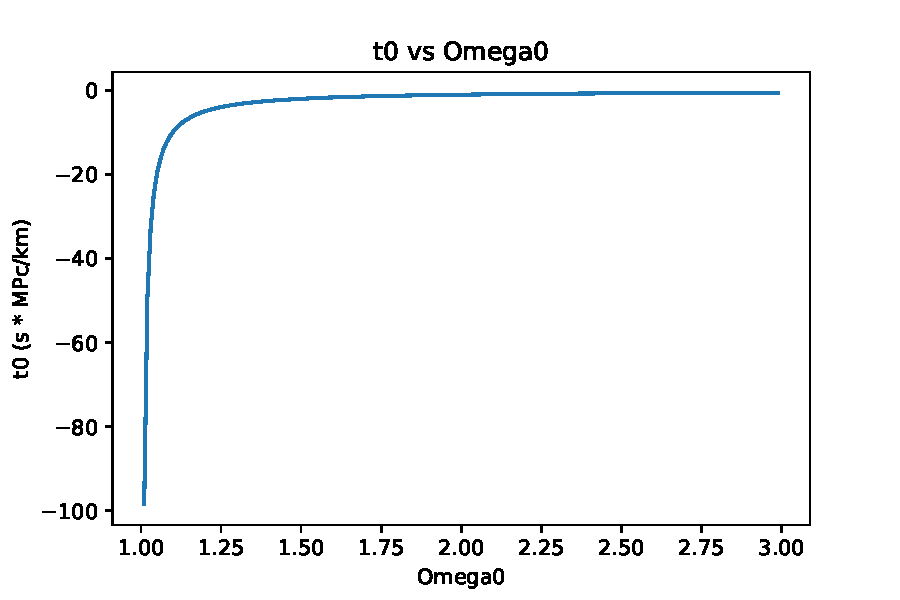
\includegraphics[scale=0.7]{Images/Q5-3.pdf}
    \caption{Plot of $t_0$ vs. $\Omega_0$ for $1 \leq \Omega_0 \leq 3$.}
    \label{plot53}
\end{figure}

\newpage 
\subsection{Present age of universe for negatively curved matter-only universe}
We recall the parametric solutions for the scale factor $a$ and the time $t$ for a negatively curved universe filled only with matter:
\begin{equation}\label{scale54}
    a(\eta) = \frac{1}{2}\frac{\Omega_0}{1 - \Omega_0}(\cosh\eta - 1)
\end{equation}
\begin{equation}\label{t54}
    t(\eta) = \frac{1}{2H_0}\frac{\Omega_0}{(1 - \Omega_0)^{3/2}}(\sinh\eta - \eta).
\end{equation}
In the present day, $a = 1$, so solving \eqref{scale54} for $\eta$ we have:
\begin{equation}
    \eta = \cosh^{-1}\left(\frac{2(1 - \Omega_0)}{\Omega_0} + 1\right) = \cosh^{-1}\left(\frac{2 - \Omega_0}{\Omega_0}\right)
\end{equation}
Substituting this into \eqref{t54} we get:
\begin{equation}
    t_0 = \frac{1}{2H_0}\frac{\Omega_0}{(1 - \Omega_0)^{3/2}}(\sinh( \cosh^{-1}\left(\frac{2 - \Omega_0}{\Omega_0}\right)) - \cosh^{-1}\left(\frac{2 - \Omega_0}{\Omega_0}\right))
\end{equation}
Now, using that $\sinh(\cosh^{-1}x) = \sqrt{x^2 - 1}$, the first term of the above expression becomes:
\begin{equation}
    \sinh( \cosh^{-1}\left(\frac{2 - \Omega_0}{\Omega_0}\right)) = \left(\frac{(2 - \Omega_0)^2}{\Omega_0^2} - 1\right)^{1/2} = \left(\frac{4 - 4\Omega_0}{\Omega_0^2}\right)^{1/2} = \frac{2}{\Omega_0}(1 - \Omega_0)^{1/2}
\end{equation}
So substituting this result we obtain:
\begin{equation}
    H_0t_0 = \frac{1}{2}\frac{\Omega_0}{(1 - \Omega_0)^{3/2}}\left(\frac{2}{\Omega_0}(1 - \Omega_0)^{1/2} - \cosh^{-1}\left(\frac{2 - \Omega_0}{\Omega_0}\right)\right)
\end{equation}
Distributing the terms, we obtain the desired result:
\begin{equation}
    \boxed{H_0t_0 = \frac{1}{1 - \Omega_0} - \frac{\Omega_0}{2(1 - \Omega_0)^{3/2}}\cosh^{-1}\left(\frac{2 - \Omega_0}{\Omega_0}\right)}.
\end{equation}
Finally, a plot of $t_0$ vs. $\Omega_0$ for $0 \leq \Omega_0 \leq 1$ is given below.

\begin{figure}[htbp]
    \centering
    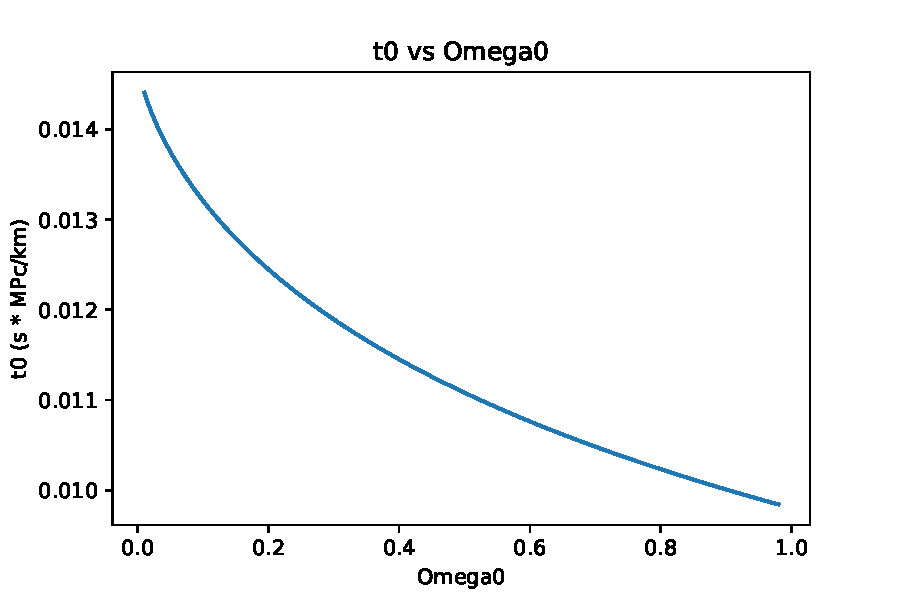
\includegraphics[scale=0.7]{Images/Q5-4.pdf}
    \caption{Plot of $t_0$ vs. $\Omega_0$ for $0 \leq \Omega_0 \leq 1$.}
    \label{plot54}
\end{figure}

\subsection{Phantom Energy and the Big Rip}
The supposed ``phantom energy'' with equation of state parameter $w_p < -1$ would have energy density:
\begin{equation}
    \e_p(a) = \e_{p, 0}a^{-3(1+w_p)}.
\end{equation}
Comparitively, matter has energy density:
\begin{equation}
    \e_{m}(a) = \e_{m, 0}a^{-3}.
\end{equation}
At equality, we have that:
\begin{equation}
    1 = \frac{\e_{p}(a)}{\e_{m}(a)} = \frac{\e_{p, 0}a^{-3(1+w_p)}}{\e_{m, 0}a^{-3}} = \frac{\Omega_{p, 0}}{\Omega_{m, 0}}\frac{1}{a^{3w_p}}
\end{equation}
Since $\Omega_{p, 0} = 1 - \Omega_{m, 0}$, we have:
\begin{equation}
    1 = \frac{1 - \Omega_{m, 0}}{\Omega_{m, 0}}\frac{1}{a^{3w_p}}
\end{equation}
Which we can rearrange to solve for the scale factor $a_{mp}$ where equality holds:
\begin{equation}
    \boxed{a_{mp} = \left(\frac{1}{\Omega_{m, 0}} - 1\right)^{1/3w_p}}
\end{equation}
The Friedmann equation in this universe reads:
\begin{equation}
    \frac{H^2}{H_0^2} = \frac{\Omega_{m, 0}}{a^3} + \frac{\Omega_{p, 0}}{a^{3(1+w_p)}} = \frac{\Omega_{m, 0}}{a^3} + \frac{1 - \Omega_{m, 0}}{a^{3(1+w_p)}}
\end{equation}
In the limit $a \gg a_{mp}$, the first term becomes negligeble and hence:
\begin{equation}
    \frac{H^2}{H_0^2} \approx \frac{1 - \Omega_{m, 0}}{a^{3(1+w_p)}}
\end{equation}
We now rearrange this equation to set up for the integration:
\begin{equation}
    \frac{\frac{\dot{a}}{a}}{H_0} \approx \frac{(1 - \Omega_{m, 0})^{1/2}}{a^{3(1+w_p)/2}} \implies H_0 dt \approx a^{3(1+w_p)/2}(1 - \Omega_{m, 0})^{-1/2}da
\end{equation}
Integrating from $t_0$ to $t_{rip}$, corresponding to from $ a(t_0) = 1$ to $a(t_{\text{rip}}) = \infty$ on the RHS, we have:
\begin{equation}
    \int_{t_0}^{t_{\text{rip}}}H_0 dt  \approx \int_1^\infty a^{3(1+w_p)/2}(1 - \Omega_{m, 0})^{-1/2}da
\end{equation}
Carrying out the integral, we get:
\begin{equation}
    H_0(t_{\text{rip}} - t_0) \approx \left. \frac{2}{3(1+w_p)}a^{3(1+w_p)/2}(1 - \Omega_{m, 0})^{-1/2}\right|_{1}^\infty
\end{equation}
Since $w_p < -1$, the RHS goes to $0$ at $a = \infty$, so:
\begin{equation}
    H_0(t_{\text{rip}} - t_0) \approx -\frac{2}{3(1+w_p)}(1 - \Omega_{m, 0})^{-1/2}
\end{equation}
Which we can write as:
\begin{equation}
    \boxed{H_0(t_{\text{rip}} - t_0) \approx \frac{2}{3\abs{1+w_p}}(1 - \Omega_{m, 0})^{-1/2}}
\end{equation}
which was the desired result. Finally, with $H_0 = 68\si{km.s^{-1}.Mpc^{-1}}, \Omega_{m, 0} = 0.3$, and $w_p = -1.1$, we can solve numerically for the time remaining until the ``Big Rip'' to be:
\begin{equation}
    \boxed{t_{\text{rip}} - t_0 \approx 2.53 \times 10^{18}\si{s} = 80.4 \times 10^{10}\si{yrs}}
\end{equation}

\subsection{Pulling an Einstein}
In this universe with matter and dark energy, the acceleration equation reads:
\begin{equation}
    \frac{\ddot{a}}{a} = -\frac{4\pi G}{3c^2}(\e + 3P) = -\frac{4\pi G}{3c^2}(\e_m + \e_q + 3w_q \e_q)
\end{equation}
Where we have used that $P = (0)\e_m = 0$ for matter and $P = w_q\e_q$ for the dark energy. To have a static universe with $\ddot{a} = 0$, it must follow that:
\begin{equation}
    \boxed{\e_m = -(1 + 3w_q)\e_q}
\end{equation}
The Friedmann equation reads:
\begin{equation}
    H(t)^2 = \frac{8\pi G}{3c^2}(\e_m + \e_q) - \frac{\kappa c^2}{R_0^2a(t)^2}
\end{equation}
Since we have a static universe, $\dot{a} = 0$ and hence $H(t) = 0$. Furthermore, using that $\e_m = -(1 + 3w_q)\e_q$ from earlier, the Friedmann equation becomes:
\begin{equation}
    0 = \frac{8\pi G}{3c^2}(-3w_q)\e_q - \frac{\kappa c^2}{R_0^2a(t)^2}
\end{equation}
Since $-1 < w_q < -1/3$, $w_q$ is negative, and hence the only way the above equality is satisfied is if $\kappa = 1$ so the positive term can be cancelled by the second term. So in this scenario, $\boxed{\text{the universe is positively curved}}$. We rearrange the above equation to solve for the radius of curvature $R_0$ when $a(t) = 1$:
\begin{equation}
    \boxed{R_0 = \sqrt{\frac{c^4}{8\pi G \abs{w_q} \e_q}}}
\end{equation}

\subsection{Big Crunch}
For a positively curved matter only universe, we recall the parametric solutions for $a(\theta), t(\theta)$ (Ryden Eqs. 5.90/5.91):
\begin{equation}
    a(\theta) = \frac{1}{2}\frac{\Omega_0}{\Omega_0 - 1}(1 - \cos\theta)
\end{equation}
\begin{equation}
    t(\theta) = \frac{1}{2H_0}\frac{\Omega_0}{(\Omega_0 - 1)^{3/2}}(\theta - \sin\theta)
\end{equation}
The big bang occurs at $\theta = 0$, and the Big crunch at $\theta = 2\pi$. Given the parametric solutions above, he time between these can be computed as (Ryden Eq. 5.92):
\begin{equation}
    t_{\text{crunch}} = \frac{\pi}{H_0}\frac{\Omega_0}{(\Omega_0 - 1)^{3/2}}
\end{equation}
Furthermore, we can solve for the present $t_0$ at which $a(\theta_0) = 1$:
\begin{equation}\label{theta0}
    a(\theta_0) = 1 = \frac{1}{2}\frac{\Omega_0}{\Omega_0 - 1}(1 - \cos\theta_0) \implies \theta_0 = \arccos\left(1 - \frac{2(\Omega_0 - 1)}{\Omega_0}\right) = \arccos\left(\frac{2}{\Omega_0} - 1\right)
\end{equation}
Therefore the time between Dr. Niwde's obsdrvations at $t = t_0 = t(\theta_0)$ and the final big crunch is given by:
\begin{equation}
    \Delta t = t_{\text{crunch}} - t(\theta_0) = \frac{\pi}{H_0}\frac{\Omega_0}{(\Omega_0 - 1)^{3/2}} - \frac{1}{2H_0}\frac{\Omega_0}{(\Omega_0 - 1)^{3/2}}(\theta_0 - \sin\theta_0)
\end{equation}
Or more concisely:
\begin{equation}
    \boxed{\Delta t = \frac{1}{H_0}\frac{\Omega}{(\Omega_0 - 1)^{3/2}}\left(\pi - \frac{1}{2}(\theta_0 - \sin\theta_0)\right)}
\end{equation}
Where $\theta_0$ is given in \eqref{theta0}. To determine the highest amplitude blueshift, we recall the redshift-scale factor relation $1 + z = \frac{1}{a}$, so:
\begin{equation}
    z = \frac{1}{a} - 1
\end{equation}
If we want to minimize $z$ (i.e. have it be the most negative/highest magnitude blueshift), we want to maximize $a$. We can determine this from the Friedmann equation (a la Ryden Eq. 5.86) but it also can easily be read off from the parametric solution above to be:
\begin{equation}
    a_{\text{max}} = \frac{\Omega_0}{\Omega_0 - 1}
\end{equation}
which is attained at $\theta = \pi$. So, the highest amplitude blueshift that Dr. Niwde can observe is at:
\begin{equation}
    \boxed{z_{\text{blue, max}} = \frac{\Omega_0 - 1}{\Omega} - 1 = -\frac{1}{\Omega_0}}
\end{equation}
At this blueshift, as stated previously we have $\theta = \pi$. So this occurs at:
\begin{equation}
    t_{\text{blue, max}} = t(\pi) =  \frac{1}{2H_0}\frac{\Omega_0}{(\Omega_0 - 1)^{3/2}}(\pi - \sin\pi) = \frac{\pi}{2H_0}\frac{\Omega_0}{(\Omega_0 - 1)^{3/2}}
\end{equation}
So the lookback time is:
\begin{equation}
   t_0 -  t_{\text{blue, max}} =  \frac{1}{2H_0}\frac{\Omega_0}{(\Omega_0 - 1)^{3/2}}(\theta_0 - \sin\theta_0) - \frac{\pi}{2H_0}\frac{\Omega_0}{(\Omega_0 - 1)^{3/2}}
\end{equation}
Or with some factoring:
\begin{equation}
    \boxed{t_0 -  t_{\text{blue, max}} = \frac{1}{2H_0}\frac{\Omega_0}{(\Omega_0 - 1)^{3/2}} \left(\theta_0 - \sin\theta_0  - 1\right)}
\end{equation}

\subsection{Big Bounce}
The Friedmann equation in such a universe would read:
\begin{equation}\label{Freid58}
    \frac{H^2}{H_0^2} = \Omega_0 + \frac{1 - \Omega_0}{a^2}
\end{equation}
At the point where $a$ has an extrema, $H(t) = 0$ and so:
\begin{equation}
    0 = \Omega_0 + \frac{1 - \Omega_0}{a^2} \implies \boxed{a_{\text{bounce}} = \left(\frac{\Omega_0 - 1}{\Omega_0}\right)^{1/2}}
\end{equation}
Rearranging the Friedmann equation, we have:
\begin{equation}
    \frac{\dot{a}}{a} = H_0\sqrt{\Omega_0}\sqrt{1 - \frac{a_{\text{bounce}}^2}{a^2}} \implies \dod{a}{t} = \frac{H_0}{\sqrt{\Omega_0}}\sqrt{a^2 - a^2_{\text{bounce}}}
\end{equation}
Integrating, we obtain:
\begin{equation}
   \sqrt{\Omega_0} H_0\int_{t_{\text{bounce}}}^{t_0} dt = \int_{a_{\text{bounce}}}^a \frac{1}{\sqrt{a'^2 - a^2_{\text{bounce}}}} da'
\end{equation}
Integrating both sides (making use of an integral table for the RHS), we have:
\begin{equation}\label{58temp}
    \sqrt{\Omega_0} H_0(t - t_{\text{bounce}}) = \arccosh\left(\frac{a}{a_{\text{bounce}}}\right)
\end{equation}
Which we can rearrange to obtain:
\begin{equation}
    \boxed{a(t) = a_{\text{bounce}}\cosh\left(\sqrt{\Omega_0} H_0(t - t_{\text{bounce}})\right)}
\end{equation}
At $t_0$ we have that $a(t_0) = 1$ by convention, so solving for $t_0 - t_{\text{bounce}}$ using \eqref{58temp} we have:
\begin{equation}
    \boxed{t_0 - t_{\text{bounce}} = \frac{1}{H_0\sqrt{\Omega_0}}\arccosh\left(\left(\frac{\Omega_0}{\Omega_0 - 1}\right)^{1/2}\right)}
\end{equation}

\subsection{$\Omega_{m, 0}$ for $t = H_0^{-1}$}
In a spatially flat and matter + cosmological constant filled universe, the Friedmann equation can be integrated to yield the analytic solution relating $t$ and $a$ (Ryden Eq. 5.101):
\begin{equation}\label{analyticmlambda}
    H_0t = \frac{2}{3\sqrt{1 - \Omega_{m, 0}}}\ln\left[\left(\frac{a}{a_{m\Lambda}}\right)^{3/2} + \sqrt{1 + \left(\frac{a}{a_{m\Lambda}}\right)^3}\right]
\end{equation}
Where $a_{m\Lambda}$ is defined by:
\begin{equation}\label{amlambda}
    a_{m\Lambda} = \left(\frac{\Omega_{m,0}}{1 - \Omega_{m, 0}}\right)^{1/3}
\end{equation}
At the present time, we have $t = t_0$, and $a = a(t_0) = 1$ by convention. Substituting this, as well as \eqref{amlambda} into \eqref{analyticmlambda} we get:
\begin{equation}
    H_0t_0 = \frac{2}{3\sqrt{1 - \Omega_{m, 0}}}\ln\left[\sqrt{\frac{1-\Omega_{m, 0}}{\Omega_{m, 0}}} + \sqrt{1 + \frac{1-\Omega_{m, 0}}{\Omega_{m, 0}}}\right]
\end{equation}
In order to have $t_0 = H_0^{-1}$ we require the RHS of the above equation to exactly equal one:
\begin{equation}
    1 = \frac{2}{3\sqrt{1 - \Omega_{m, 0}}}\ln\left[\sqrt{\frac{1-\Omega_{m, 0}}{\Omega_{m, 0}}} + \sqrt{1 + \frac{1-\Omega_{m, 0}}{\Omega_{m, 0}}}\right]
\end{equation}
Rewriting the last term:
\begin{equation}
    1 = \frac{2}{3\sqrt{1 - \Omega_{m, 0}}}\ln\left[\sqrt{\frac{1-\Omega_{m, 0}}{\Omega_{m, 0}}} + \sqrt{\frac{1}{\Omega_{m, 0}}}\right] = \frac{2}{3\sqrt{1 - \Omega_{m, 0}}}\ln\left[\frac{1 + \sqrt{1 - \Omega_{m, 0}}}{\sqrt{\Omega_{m, 0}}}\right]
\end{equation}
Using the hyperbolic secant identity of $\arcsech x = \ln(\frac{1 + \sqrt{1 - x^2}}{x})$, we have:
\begin{equation}
    1 = \frac{2}{3\sqrt{1 - \Omega_{m, 0}}}\arcsech(\sqrt{\Omega_{m, 0}})
\end{equation}
Or:
\begin{equation}\label{59exp}
    \frac{3\sqrt{1 - \Omega_{m, 0}}}{2} = \arcsech(\sqrt{\Omega_{m, 0}})
\end{equation}
This equation can now be solved numerically for $\Omega_{m, 0}$ to find:
\begin{equation}
    \boxed{\Omega_{m, 0} \approx 0.263}
\end{equation}

\subsection{Amounts in the Benchmark model}
In the Benchmark model, we have (from Ryden Table 5.2) that:
\begin{equation}
    \Omega_{m, 0} = 0.31, \quad \Omega_{\gamma, 0} = 5.35 \times 10^{-5},\quad  \Omega_{\text{bary}, 0} = 0.048
\end{equation}
We that $\Omega = \frac{\e(t)}{\e_c(t)}$ where $\e_C$ is the critical density, which is currently $\e_{c, 0} 7.8 \times 10^{-10}\si{J.m^{-3}}$ (up to uncertainty). Therefore obtaining the energy density for photons in the benchmark model, we have:
\begin{equation}
    \e_{\gamma, 0} = \e_{c, 0}\Omega_{\gamma, 0} = 4.17 \times 10^{-14} \si{J.m^{-3}}
\end{equation}
It will be more convenient to solve for the mass density for the matter and baryons:
\begin{equation}
    \rho_{m, 0} = \e_{c, 0}\Omega_{\gamma, 0}/c^2 = 2.69 \times 10^{-27}\si{kg.m^{-3}}, \quad \rho_{\text{bary}, 0} = \e_{c, 0}\Omega_{\text{bary}, 0}/c^2 = 4.16 \times 10^{-28} \si{J.m^{-3}} 
\end{equation}
In addition, in the Benchmark model we have a finite horizon distance (Ryden Eq. 5.115):
\begin{equation}
    d_{\text{hor}}(t_0) = 14000\si{Mpc} = 4.33 \times 10^{26}\si{m}.
\end{equation}
Therefore the volume of the universe within the horizon distance is:
\begin{equation}
    V_{\text{hor}}(t_0) = \frac{4}{3}\pi d_{\text{hor}}(t_0)^3 = 3.39 \times 10^{80} \si{m^3}
\end{equation}
Now, solving for the total mass of all matter within our horizon, we have:
\begin{equation}
    \boxed{M_m =  V_{\text{hor}}(t_0)\rho_{m, 0} = 9.12 \times 10^{53}\si{kg}}
\end{equation}
Next, solving for the total amount of energy of photons within the horizon distance, we have:
\begin{equation}
    \boxed{E_{\text{photons}} = V_{\text{hor}}(t_0)\e_{\gamma, 0} = 1.41 \times 10^{67} \si{J}}
\end{equation}
Finally, we solve for the number of baryons in the universe. This will be the total mass of baryons within the universe divided by the mean mass per Baryon, which we take to be the mass of a proton $m_p$. Therefore the total number of baryons within the horizon can be solved for as:
\begin{equation}
    \boxed{N_{\text{bary}} =  V_{\text{hor}}(t_0)\rho_{\text{bary}, 0}/m_{p} = 8.45 \times 10^{79} \text{baryons}}
\end{equation}

\subsection*{Time and Scale Factor for Matter-Only Universe}
\addcontentsline{toc}{subsection}{\protect\numberline{}Time and Scale Factor for Matter-Only Universe}
\begin{tcolorbox}
Let's make sure we can work through the mathematical steps for a closed matter-only (i.e. `Matter + Curvature') universe. Try to do this without looking up the book for every step! Start by writing the Friedmann equation for this case, using $a$ rather than $1+z$, and with the single parameter $\Omega_0$ (where this implicitly means `matter', here). Thus write an integral expression for $t$. It may not look trivial to solve this for $t(a)$ or $a(t)$, but you should be able to \emph{show} that the following parametric solution works [a `parametric solution' means that you can write doesn $y(\phi)$ and $x(\phi)$, both in terms of a parameter $\phi$, even if an explicit expression for $y(x)$ is hard or impossible]:
\begin{equation}\label{parametric_a}
    a(\theta) = \frac{1}{2}\frac{\Omega_0}{\Omega_0 - 1}(1-\cos\theta)
\end{equation}
\begin{equation}\label{parametric_t}
    t(\theta) = \frac{1}{2H_0}\frac{\Omega_0}{(\Omega_0 - 1)^{3/2}}(\theta - \sin\theta).
\end{equation}
To be clear: you are being asked to show that in the appropriate Friedmann equation, the LHS is equal to the RHS if you assume the above solution (\emph{or} you could solve the integral, but that's harder!). [You might have to do a bit of rearranging of trig functions - but perservere, because it works!] Lastly, by letting $\theta$ run from $0$ to $2\pi$, sketch $a$ vs. $t$ for this model. 
\end{tcolorbox}

The Friedmann equation in this case reads:
\begin{equation}
    \boxed{\frac{H^2}{H_0^2} = \frac{\Omega_0}{a^3} + \frac{1 - \Omega_0}{a^2}}
\end{equation}
Now, since $H = \frac{\dot{a}}{a}$, we can rearrange this to obtain that:
\begin{equation}\label{friedmann_mat}
    \frac{\dot{a}^2}{H_0^2} = (\frac{\Omega_0}{a} + 1 - \Omega_0)
\end{equation}
Or in other words:
\begin{equation}
    \dod{a}{t} = H_0\sqrt{\frac{\Omega_0}{a} + 1 - \Omega_0}
\end{equation}
So solving for $t$ we integrate:
\begin{equation}
    \boxed{H_0t = \int_0^t dt' = \int_0^a \frac{da'}{\sqrt{\frac{\Omega_0}{a} + 1 - \Omega_0}}}.
\end{equation}
Now, we verify that \eqref{friedmann_mat} holds for the parametric solution given by \eqref{parametric_a} and \eqref{parametric_t}. First, we determine what $\dot{a}$ is given this solution. By the chain rule, we have that:
\begin{equation}
    \dot{a} = \dod{a}{t} = \dod{a}{\theta}\dod{\theta}{t} = \dod{a}{\theta}\dot{\theta}
\end{equation}
Solving for $\od{a}{\theta}$ by differentiating \eqref{parametric_a} we have:
\begin{equation}
    \dod{a}{\theta} = \frac{1}{2}\frac{\Omega_0}{\Omega_0 - 1}\sin\theta.
\end{equation}
And solving for $\dot{theta}$ by implicitly differentiating \eqref{parametric_t} we have:
\begin{equation}
    1 = \frac{1}{2H_0}\frac{\Omega_0}{(\Omega_0 - 1)^{3/2}}(\dot{\theta} - \dot{\theta}\cos\theta) \implies \dot{\theta} = \frac{2H_0(\Omega_0 - 1)^{3/2}}{\Omega_0(1-\cos\theta)}
\end{equation}
Hence, we find that:
\begin{equation}
    \dot{a} = \frac{H_0(\Omega_0 - 1)^{1/2}}{1 - \cos\theta}\sin\theta
\end{equation}
Evaluating the LHS of \eqref{friedmann_mat}, we have:
\begin{equation}\label{LHS_friedmann_mat}
    \frac{\dot{a}^2}{H_0^2} = \frac{\Omega_0 - 1}{(1 - \cos\theta)^2}\sin^2\theta
\end{equation}
Evaluating the RHS of \eqref{friedmann_mat}, we have:
\begin{equation}
    \frac{\Omega_0}{a} + 1 - \Omega_0 = (\frac{\Omega_0}{\frac{1}{2}\frac{\Omega_0}{\Omega_1 - 1}(1-\cos\theta)} + 1 - \Omega_0)
\end{equation}
Multiplying the first term by $1 = \frac{1 - \cos\theta}{1-\cos\theta}$ and the second term by $1 = \left(\frac{1 - \cos\theta}{1-\cos\theta}\right)^2$ we obtain:
\begin{equation}
    \frac{\Omega_0}{a} + 1 - \Omega_0 = \frac{2(\Omega_0 - 1)}{(1 -\cos\theta)^2}(1 - \cos\theta) - \frac{\Omega_0 - 1}{(1 - \cos\theta)^2}(1 - \cos\theta)^2
\end{equation}
Which after some expanding and cancellation, becomes:
\begin{equation}\label{RHS_friedmann_mat}
    \frac{\Omega_0}{a} + 1 - \Omega_0 = \frac{\Omega_0 - 1}{(1 - \cos\theta)^2}(1 -\cos^2\theta)
\end{equation}
Using the famous trig identity $\sin^2\theta + \cos^2\theta = 1$, we can identify \eqref{LHS_friedmann_mat} with \eqref{RHS_friedmann_mat} to conclude that this is indeed the correct solution.

For the plot, we observe that the given parametric equations are exactly of those for a cycloid, so the curve of $t(\theta)$ vs. $a(\theta)$ will be exactly that it is displayed below.

\begin{figure}[htbp]
    \centering
    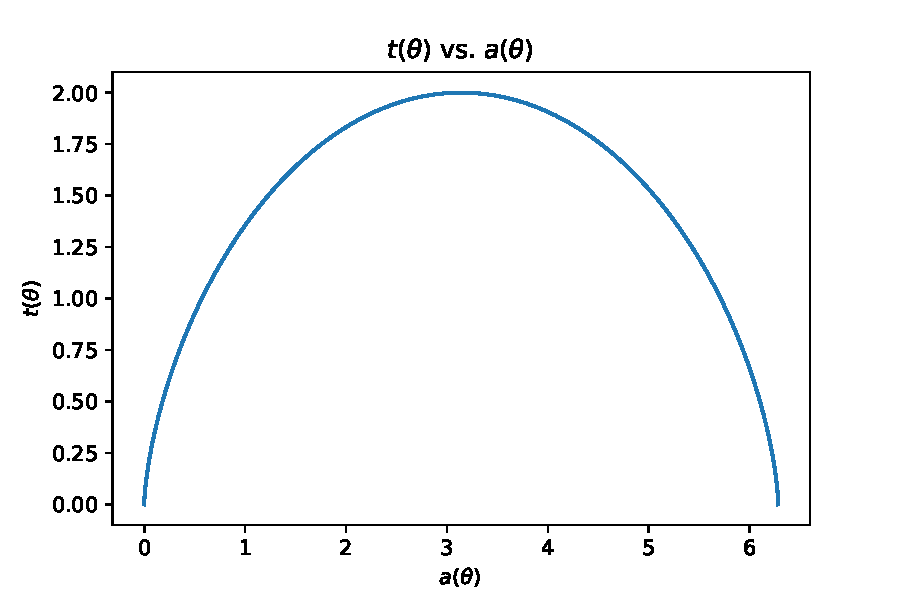
\includegraphics[scale=0.7]{Images/Q5-A.pdf}
    \caption{Plot of $t(\theta)$ vs. $a(\theta)$ for $\theta \in [0, 2\pi)$. $\Omega_0 = 2$ and $H_0 = 1$ were chosen for convenience of plotting.}
    \label{plotatcycloid}
\end{figure}
\newpage
\section[Measuring Cosmological Parameters]{\hyperlink{toc}{Measuring Cosmological Parameters}}

\subsection{Magnitudes and Polar Bear Feet}
First solving for the bolometric absolute magnitude of the bear's foot, we have:
\begin{equation}
    M_B = -2.5\log_{10}\left(\frac{L}{L_x}\right) = -2.5\log_{10}\left(\frac{10 \si{W}}{78.7 L_{\odot}}\right) = -2.5\log_{10}\left(\frac{10 \si{W}}{78.7 \cdot 3.82 \times 10^{26} \si{W}}\right) 
\end{equation}
Numerically, this is:
\begin{equation}
    \boxed{M_B = 68.7}
\end{equation}
Now for the apparent magnitude at luminosity distance of $d_L = 0.5\si{km}$. We first calculate the flux of the polar bear foot to be
\begin{equation}
    f_B \frac{L}{4\pi d_L^2} = \frac{10\si{W}}{4 \pi(500\si{m})^2} = 3.18 \times 10^{-6} \si{W m^{-2}}
\end{equation}
So therefore calculating the apparent magnitude, we have:
\begin{equation}
    m_B = -2.5\log_{10}\left(\frac{f_B}{f_x}\right) = -2.5\log_{10}\left(\frac{3.18 \times 10^{-6} \si{W m^{-2}}}{2.53 \times 10^{-8} \si{Wm^{-2}} }\right)
\end{equation}
Which numerically we calculate to be:
\begin{equation}
    \boxed{m_B = -5.25}
\end{equation}
If we have a bolometer that can detect the the bear's foot at a maximum luminosity distance of $d_L = 0.5\si{km}$, then $f_B$ (the flux of the bear foot at this distance) defines the maximum flux $f_{\text{max}}$ that is capable of being detected, so solving for the maximum luminosity distance it could detect the sun, we have:
\begin{equation}
    \boxed{d_{\text{max, sun}} = \sqrt{\frac{L_\odot}{4\pi f_{\text{max}}}} = 3.09 \times 10^{15}\si{m}}
\end{equation}
Repeating this calculation for the supernova, we have:
\begin{equation}
    \boxed{d_{\text{max, supernova}} = \sqrt{\frac{L_{\text{supernova}}}{4\pi f_{\text{max}}}} = \sqrt{\frac{4 \times 10^9 L_\odot}{4\pi f_{\text{max}}}} = 1.96 \times 10^{20}\si{m}}
\end{equation}


\subsection{Angular Size and Polar Bear Feet}
We know that:
\begin{equation}
    d_A = \frac{l}{\delta \theta}
\end{equation}
so given $l = 0.16\si{m}$ and $d_A = 0.5\si{km}$, we can rearrange to solve for the angular size to be:
\begin{equation}
    \boxed{\delta \theta = \frac{l}{d_A} = \frac{0.16\si{m}}{500\si{m}} = 3.2 \times 10^{-4}\si{rad}}
\end{equation}
The critical redshift of the benchmark model is $z_C = 1.6$, where $d_{A, \text{max}} = 5.31 \times 10^{25}\si{m}$, so:
\begin{equation}
    \boxed{\delta \theta_{\text{max}} = \frac{l}{d_{A, \text{max}}} = 3 \times 10^{-27}\si{rad}}
\end{equation}


\subsection{Maximizing $d_A$ in a flat, single-component universe}
In a spatially flat, single-component universe, the scale factor is given as (Ryden Eq. 5.39):
\begin{equation}
    a(t) = \left(\frac{t}{t_0}\right)^{2/(3 + 3w)}
\end{equation}
So we can integrate to obtain the proper distance (Ryden Eq. 5.49):
\begin{equation}\label{dpt063int}
    d_p(t_0) = c\int_{t_e}^{t_0}\frac{dt}{a(t)} = c\int_{t_e}^{t_0}\left(\frac{t}{t_0}\right)^{-2/(3 + 3w)}dt = ct_0\frac{3(1 + w)}{1 + 3w}\left[1 - (t_e/t_0)^{(1+3w)/(3+3w)}\right]
\end{equation}
Furthermore, using that $1 + z = \frac{a(t_0)}{a(t_e)} = (t_0/t_e)^{2/(3+3w)}$ (Ryden Eq. 5.47) to find $t_e$, we obtain (Ryden Eq. 5.48):
\begin{equation}
    t_e = \frac{t_0}{(1+z)^{(3+3w)/2}} = \frac{2}{3(1+w)H_0}\frac{1}{(1+z)^{3(1+w)/2}}
\end{equation}
Substituting this into \eqref{dpt0int} we find the current proper distance in terms of $z$:
\begin{equation}
    \boxed{d_p(t_0) = \frac{c}{H_0}\frac{2}{1+3w}\left[1 - (1+z)^{-(1+3w)/2}\right]}
\end{equation}
Further, in the case of a spatially flat universe, we can use Ryden Eq. 6.37 to obtain the current angular and luminosity distances:
\begin{equation}\label{da63}
    \boxed{d_A(t_0) = \frac{d_p(t_0)}{1+z} =  \frac{c}{H_0}\frac{2}{1+3w}\left[1 - (1+z)^{-(1+3w)/2}\right]\frac{1}{1+z}}
\end{equation}
\begin{equation}
    \boxed{d_L(t_0) = d_p(t_0)(1+z) = \frac{c}{H_0}\frac{2}{1+3w}\left[1 - (1+z)^{-(1+3w)/2}\right](1+z)}
\end{equation}
To solve for the critical redshift $z_C$ where $d_A$ has the maximum value, we take the derivative of \eqref{da63} with respect to $z$ and set it to 0:
\begin{equation}
    \dod{d_A}{z} =  \frac{c}{H_0}\frac{2}{1+3w}\left(-(1+z)^{-2} + \frac{3+3w}{2}(1+z)^{-(5+3w)/2}\right) = 0
\end{equation}
The terms in the brackets must vanish, so:
\begin{equation}
    -(1+z)^{-2} + \frac{3+3w}{2}(1+z)^{-(5+3w)/2} = 0
\end{equation}
Cancelling out a factor of $(1+z)^{-2}$, we get:
\begin{equation}
    \frac{3+3w}{2}(1+z)^{-(1+3w)/2} = 1
\end{equation}
Now rearranging to solve for $z_c$, we find:
\begin{equation}
    \boxed{z_c = \left(\frac{2}{3+3w}\right)^{(1+3w)/2} - 1}
\end{equation}
We can now substitute this back into \eqref{da63} to find what the maximum redshift is:
\begin{multline}
    d_{A, \text{max}} =  \frac{c}{H_0}\frac{2}{1+3w}\left[1 - (1+z_c)^{-(1+3w)/2}\right]\frac{1}{1+z_c}
    \\ = \frac{c}{H_0}\frac{2}{1+3w}\left[1 - \left(\left(\frac{2}{3+3w}\right)^{(1+3w)/2}\right)^{-(1+3w)/2}\right]\left(\frac{2}{3+3w}\right)^{-(1+3w)/2}
\end{multline}
So we conclude:
\begin{equation}
    \boxed{d_{A, \text{max}} = \frac{c}{H_0}\frac{2}{1+3w}\left[1 - \left(\frac{2}{3+3w}\right)^{-(1+3w)^2/4}\right]\left(\frac{2}{3+3w}\right)^{-(1+3w)/2}}
\end{equation}

\subsection{Difference between relative and absolute magnitude}
At small redshift ($z \ll 1$), the luminosity distance is approximately (Ryden Eq. 6.50, also seen in class):
\begin{equation}
    d_L \approx \frac{c}{H_0}z\left(1 + \frac{1 - q_0}{2}z\right).
\end{equation}
By Ryden Eq 6.49, the distance modulus is given by:
\begin{equation}
    m - M = 5\log_{10}\left(\frac{d_L}{1\si{Mpc}}\right) + 25.
\end{equation}
Substituting the first equation into the second, we get:
\begin{equation}
    m - M \approx 5\log_{10}\left(\frac{\frac{c}{H_0}z\left(1 + \frac{1 - q_0}{2}z\right)}{1\si{Mpc}}\right) +  25
\end{equation}
From here on out, we will supress the $1\si{Mpc}$ in the denominator for clarity:
\begin{equation}
    m - M \approx 5\log_{10}\left(\frac{c}{H_0}z\left(1 + \frac{1 - q_0}{2}z\right)\right) +  25
\end{equation}
Using that $\log(ab) = \log(a) + \log(b)$ we get:
\begin{equation}
    m - M \approx 5\log_{10}\left(\frac{c}{H_0}z\right) + 5\log_{10}\left(1 + \frac{1 - q_0}{2}z\right) +  25
\end{equation}
Using the approximation $\log_{10}(1 + x) \approx 0.4343\ln(1 + x) \approx 0.4343x$ for small $x$ on the second term, we get:
\begin{equation}
    m - M \approx 5\log_{10}\left(\frac{c}{H_0}z\right) + 5(0.4343)(\frac{1 - q_0}{2}z) +  25 
\end{equation}
Simplifying the numerical terms in the second term, and multiplying by one in the argument of the first term, we get:
\begin{equation}
    m - M \approx 5\log_{10}\left(\frac{c}{H_0}z \frac{68 \si{km.s^{-1}.Mpc^{-1}}}{68 \si{km.s^{-1}.Mpc^{-1}}}\right) + 1.086(1-q_0)z +  25 
\end{equation}
Further application of the $\log(ab) = \log(a) + \log(b)$ rule yields:
\begin{equation}
    m - M \approx 5\log_{10}\left(\frac{c}{68 \si{km.s^{-1}.Mpc^{-1}}}\right) + 5\log_{10}z + 5\log_{10}\left(\frac{68 \si{km.s^{-1}.Mpc^{-1}}}{H_0}\right) + 1.086(1-q_0)z +  25
\end{equation}
Applying the $\log(\frac{1}{x}) = -\log(x)$ rule we get:
\begin{equation}
    m - M \approx 5\log_{10}\left(\frac{c}{68 \si{km.s^{-1}.Mpc^{-1}}}\right) + 5\log_{10}z - 5\log_{10}\left(\frac{H_0}{68 \si{km.s^{-1}.Mpc^{-1}}}\right) + 1.086(1-q_0)z +  25
\end{equation}
Before we evaluate the first term numerically, we recall the supressed $\si{Mpc}$, so:
\begin{equation}
    m - M \approx 5\log_{10}\left(\frac{300000\si{km.s^{-1}}}{68 \si{km.s^{-1}}}\right) + 5\log_{10}z - 5\log_{10}\left(\frac{H_0}{68 \si{km.s^{-1}.Mpc^{-1}}}\right) + 1.086(1-q_0)z +  25
\end{equation}
We use a calculator to check the value of the first term:
\begin{equation}
    m - M \approx 5(3.6446) + 5\log_{10}z - 5\log_{10}\left(\frac{H_0}{68 \si{km.s^{-1}.Mpc^{-1}}}\right) + 1.086(1-q_0)z +  25
\end{equation}
Grouping the numerical terms:
\begin{equation}
    \boxed{m - M \approx 43.23 - 5\log_{10}\left(\frac{H_0}{68 \si{km.s^{-1}.Mpc^{-1}}}\right) + 5\log_{10}z + 1.086(1-q_0)z}.
\end{equation}

\subsection{Surface Brightness}
First, we recall the angular diameter distance $d_A$ to a standard yardstick to be (Ryden Eq. 6.35):
\begin{equation}
    d_A \equiv \frac{l}{\delta \theta} = \frac{S_\kappa(r)}{1 + z}
\end{equation}
Rearranging, we find:
\begin{equation}
    \delta \theta = \frac{l(1 + z)}{S_\kappa(r)}
\end{equation}
The observed flux is related to the luminosity $L$ and the observed flux $f$ as (Ryden 6.27):
\begin{equation}
    f = \frac{L}{4\pi S_\kappa(r)^2 (1+z)^2}
\end{equation}
So, $\Sigma$ as a function of redshift is:
\begin{equation}
    \Sigma \propto \frac{f}{(\delta \theta)^2} = \frac{\frac{L}{4\pi S_\kappa(r)^2 (1+z)^2}}{\left(\frac{l(1 + z)}{S_\kappa(r)}\right)^2} = \frac{L}{l^2 4\pi} \frac{1}{(1+z)^4} \propto \frac{1}{(1+z)^4}
\end{equation}
So:
\begin{equation}
    \boxed{\Sigma = \frac{\Sigma_0}{(1+ z)^4}}
\end{equation}
for some constant $\Sigma_0$. Since the surface brightness $\Sigma$ only depends on the redshift and not cosmological parameters, $\boxed{\text{we cannot use it to measure a cosmological parameter $q_0$}}$.

\subsection{Quasar Light Flux}
The variation time scale at the time light was emitted is related to the variation timescale when it was observed via:
\begin{equation}
    \delta t_0 = (1 + z)\delta t_e
\end{equation}
So for redshift $z = 5.0$ and $\delta t_0$ of 3 days, the variation time scale when emitted is:
\begin{equation}
    \boxed{\delta t_e = 0.5 \si{days}}
\end{equation}
$R_{\text{max}}$ for the observed quasar is:
\begin{equation}
    \boxed{R_{\text{max}} = c(\delta t_e) = 6.48 \times 10^{12} \si{m}}
\end{equation}
From Ryden Figure 6.4, a standard yardstick with redshift $z = 5.0$ has angular distance $d_A \approx 0.3c/H_0$ in the Benchmark model, so the angular size is given by:
\begin{equation}
    \boxed{\delta \theta = \frac{R_{\text{max}}}{d_A} = \frac{6.48 \times 10^{12} \si{m}}{0.3c/H_0} = 1.58 \times 10^{-44}\si{rad}}
\end{equation}


\subsection{Proper Area of a sphere}
The FRW metric (Ryden Eq. 6.22) is:
\begin{equation}
    ds^2 = -c^2dt^2 + a(t)^2[dr^2 + S_k(r)^2d\Omega^2]
\end{equation}
Expanding out $d\Omega$, this becomes:
\begin{equation}
    ds^2 = -c^2dt^2 + a(t)^2[dr^2 + S_k(r)^2d\theta^2 + S_\kappa(r)^2\sin^2\theta d\phi^2]
\end{equation}
For a space described by this metric, a surface element $dA$ on a sphere of radius $r$ will be given by:
\begin{equation}
    dA = (S_\kappa(r)d\theta)(S_\kappa(r)\sin\theta d\phi) = S_\kappa(r)^2 \sin\theta d\theta d\phi
\end{equation}
Integrating this surface area to find the surface area of this sphere, we have:
\begin{equation}
    A = \iint dA = \iint S_\kappa(r)^2 \sin\theta d\theta d\phi = S_\kappa(r)^2 \int_{0}^{\pi}\sin\theta d\theta \int_{0}^{2\pi}d\phi = S_\kappa(r)^2(2)(2\pi) = 4\pi S_\kappa(r)^2
\end{equation}
Therefore setting $r$ to be the proper radius $r = d_p(t_0)$, we obtain:
\begin{equation}
    \boxed{A_p(t_0) = 4\pi S_\kappa(r)^2}.
\end{equation}

\subsection{Total Intensity of Standard Candles}
The relation between the observed flux $f$ and the Luminosity $L$ of a distant light source is given by:
\begin{equation}
    f = \frac{L}{4\pi S_\kappa(r)^2(1+z)^2}
\end{equation}
Since we live in a flat universe, $S_\kappa(r) = r$ and so:
\begin{equation}\label{flux68}
    f = \frac{L}{4\pi r^2(1+z)^2}
\end{equation}
In a single-component universe, the proper distance $r = d_p(t_0)$ for $w \neq -1/3$ is given by (Ryden Eq 5.50):
\begin{equation}
    r = d_p(t_0) = \frac{c}{H_0}\frac{2}{1+3w}\left[1 - (1+z)^{-(1+3w)/2}\right]
\end{equation}
So subsituting this into \eqref{flux68} we have:
\begin{equation}
    f(z) = \frac{L}{4\pi \left(\frac{c}{H_0}\frac{2}{1+3w}\left[1 - (1+z)^{-(1+3w)/2}\right]\right)^2(1+z)^2}
\end{equation}
Which we can rewrite as:
\begin{equation}
    \boxed{f(z) = \frac{L(1+3w)^2}{16\pi(c/H_0)^2}\frac{1}{(1+z)^2}\left[1 - (1+z)^{-(1+3w)/2}\right]^{-2}}
\end{equation}
which was the desired expression. When $w = -1/3$, the scale factor in a spatially flat, single component universe is given by:
\begin{equation}
    a(t) = \left(\frac{t}{t_0}\right)^{2/(3+3w)} = \left(\frac{t}{t_0}\right)^{2/(3-1)} = \frac{t}{t_0}
\end{equation}
Therefore, the Hubble constant is given by:
\begin{equation}
    H_0 = \left.\frac{\dot{a}}{a}\right|_{t = t_0} = \frac{\frac{1}{t_0}}{\frac{t_0}{t_0}} = \frac{1}{t_0}
\end{equation}
The redshift is given by:
\begin{equation}
    1 + z = \left(\frac{t_0}{t_e}\right)^{2/(3+3w)} = \frac{t_0}{t_e}
\end{equation}
Solving for the proper distance $r = d_p(t_0)$ in this universe, we have:
\begin{equation}
    r = d_p(t_0) = c\int_{t_e}^{t_0}\frac{\mathrm d t}{a(t)} = ct_0\int_{t_e}^{t_0} \frac{\mathrm d t}{t} = ct_0\ln(\frac{t_0}{t_e}) = \frac{c}{H_0}\ln(1+z)
\end{equation}
Therefore the observed flux in this universe is given by:
\begin{equation}\label{wneg13}
    \boxed{f(z) = \frac{L}{4\pi(c/H_0)^2\ln^2(1+z)}\frac{1}{(1+z)^2}}
\end{equation}
The number of stars located in the range $r$ to $r + \mathrm d r$ in the sky per steradian will be given by:
\begin{equation}
    N(r) = n_0 r^2 dr
\end{equation}
So the number of stars in the range $z$ to $z + \mathrm d z$ per steradian is given by:
\begin{equation}
    N(z) = n_0 r^2 \dod{}{z}\left(\frac{c}{H_0}\frac{2}{1+3w}\left[1 - (1+z)^{-(1+3w)/2}\right]\right)
\end{equation}
Taking the derivative:
\begin{equation}
    N(z) =  n_0 r^2 \left(\frac{c}{H_0}(1+z)^{-(3 + 3w)/2}\right)\mathrm d z
\end{equation}
So, finding the intensity from standard candles in the range $z$ to $z + \mathrm d z$, we multiply the earlier result for $f(z)$ with the above result for $N(z)$:
\begin{equation}
    \mathrm d J(z) = f(z)N(z) = \frac{L}{4\pi r^2(1+z)^2} n_0 r^2\left(\frac{c}{H_0}(1+z)^{-(3 + 3w)/2}\right)\mathrm d z
\end{equation}
Which after cancelling terms:
\begin{equation}
    \boxed{\mathrm d J(z) = \frac{n_0L(c/H_0)}{4\pi}(1+z)^{-(7+3w)/2}\mathrm d z}
\end{equation}
which is the desired result. To find the total intensity $J$, we integrate over all redshifts:
\begin{equation}
    J = \int_0^\infty \mathrm d J(z) = \int_0^\infty  \frac{n_0L(c/H_0)}{4\pi}(1+z)^{-(7+3w)/2}\mathrm d z =   \left.\frac{n_0L(c/H_0)}{4\pi}\frac{-2}{(1+3w)}(1+z)^{-(5+3w)/2}\right|_0^\infty
\end{equation}
This gives us the result:
\begin{equation}
    J = \begin{cases}
        \frac{n_0 L(c/H_0)}{4\pi}\frac{1 + 3w}{2} & w > -\frac{5}{3}
        \\ \infty & w < -\frac{5}{3}
    \end{cases}
\end{equation}
To obtain the $w = -\frac{1}{3}$ result, we would have to repeat the analysis using \eqref{wneg13}, but we leave this as an exercise.

The result above tells us that the total intensity we have in a universe with $w < -\frac{5}{3}$ is infinite! On some level this makes sense, as the horizon distance is infinite. However, in this universe, we claim the apparently paradoxical result that the brightness of the night sky is still finite. Why? Because the above calculation assumes that we see light flux from every single standard candle in the universe; this is simply NOT the case. There will be standard candles that block the sight of other standard candles to ours, so we simply do not see the light from every light source in the universe (and hence the above result is actually misleading, as it does not take into account the fact that light sources block other light sources). The maximum possible brightness we could have is if stars paved the sky (i.e. every sightline was blocked eventually by a star). In this scenario, we can repeat the calculation as done in Chapter 2 of Ryden. If a standard candle of radius $R_*$ is at a distance $r \gg R_*$, its angular area in steradians is given by:
\begin{equation}
    \Omega = \frac{\pi R_*^2}{4\pi r^2 (1+z)^2} = \frac{R_*^2}{4r^2(1+z)^2}
\end{equation}
and its measured flux will be:
\begin{equation}
    f = \frac{L_*}{4\pi r^2(1+z)^2}
\end{equation}
so the surface brightness of the star, in watts per square meter is:
\begin{equation}
    \Sigma_* = \frac{f}{\Omega} = \frac{L_*}{\pi R_*^2}
\end{equation}
which also gives the surface brightness of the paved sky, which while large, is most certainly finite!

\subsection{Expansion Switch}
The acceleration equation can be written as:
\begin{equation}
    -\frac{\ddot{a}}{aH^2} = \frac{1}{2}\sum_{i=1}^N \Omega_i(1+3w_i)
\end{equation}
where the sum is taken over the different components of the universe. In the Benchmark model, we have matter $(w = 0)$, radiation $(w = \frac{1}{3})$, and the cosmological constant $(w = -1)$, and so:
\begin{equation}
    -\frac{\ddot{a}}{aH^2} = \frac{1}{2}\Omega_m + \Omega_r - \Omega_\Lambda
\end{equation}
We have that $\Omega_m = \frac{\Omega_{m, 0}}{a^3}, \Omega_r = \frac{\Omega_{r, 0}}{a^4}$, and $\Omega_\Lambda = \Omega_{\Lambda, 0}$, so:
\begin{equation}
    -\frac{\ddot{a}}{aH^2} = \frac{1}{2}\frac{\Omega_{m, 0}}{a^3} + \frac{\Omega_{r, 0}}{a^4} - \Omega_{\Lambda, 0}
\end{equation}
Setting $\ddot{a}$ to find the scale factor $a$ for which the expansion of the universe switched from slowing down to speeding up, we have:
\begin{equation}
    0 =  \frac{1}{2}\frac{\Omega_{m, 0}}{a^3} + \frac{\Omega_{r, 0}}{a^4} - \Omega_{\Lambda, 0}
\end{equation}
Multiplying by $a^4$ we get:
\begin{equation}
    0 = \frac{1}{2}\Omega_{m, 0}a + \Omega_{r, 0} - \Omega_{\Lambda, 0}a^4
\end{equation}
In the Benchmark model, $\Omega_{m, 0} = 0.31, \Omega_{r, 0} = 9.0 \times 10^{-5}$, and $\Omega_{\Lambda, 0} \approx 0.69$. The radiation term can be neglected to good approximation, yielding:
\begin{equation}
    0 \approx a(\frac{1}{2}\Omega_{m, 0} - \Omega_{\Lambda, 0}a^3)
\end{equation}
So solving for the positive root of this equation, we get:
\begin{equation}
    \boxed{a = \sqrt[3]{\frac{\Omega_{m, 0}}{2\Omega_{\Lambda, 0}}} \approx 0.608}
\end{equation}
Which we note is $\boxed{\text{less}}$ than the scale factor at matter-lambda equality of $a_{m\Lambda} = 0.77$. 
\newpage
\section[Dark Matter]{\hyperlink{toc}{Dark Matter}}

\subsection{Dark Matter Candidates}
Taking the radius of the halo to be $R_{\text{halo}} \approx 75 \si{kpc}$ and the mass of our galaxy to be $M_{\text{gal}} \approx 9.6 \times 10^{11} M_\odot$, we approximate that roughly all of the mass comes from dark matter, hence giving us $N = M_{\text{gal}}/10^{-8}M_\odot = 9.6 \times 10^{19}$ black holes. The volume of our galaxy is given by:
\begin{equation}
    V = \frac{4}{3}\pi R_{\text{halo}}^3 = 5.2 \times 10^{64}\si{m^3}
\end{equation}
The number density of these black holes in our galaxy is therefore given by:
\begin{equation}
    n_{\text{BH}} = \frac{N}{V} = \frac{9.6 \times 10^{19}}{5.2 \times 10^{64}\si{m^3}} \approx 1.85 \times 10^{-42} \si{m^{-3}}
\end{equation}
In other words, we can find one black hole per:
\begin{equation}
    V_{\text{BH}} = \frac{1}{n_{BH}} = 5.4 \times 10^{41}\si{m^3}
\end{equation}
So the nearest black hole would (approximately) be a distance of:
\begin{equation}
    \boxed{d_{\text{BH}} \approx \sqrt[3]{V_{BH}} = 8.1 \times 10^{13}\si{m}}
\end{equation}
away. The mean free path before a black hole comes into a distance $1 \si{AU}$ with our sun is given by:
\begin{equation}
    \lambda_{\text{BH}} = \frac{1}{n_{BH}\sigma} = \frac{1}{n_{BH}\pi (1 \si{AU})^2} = 7.6 \times 10^{18}\si{m}
\end{equation}
So combining this with the solar galactic orbital speed of $235 \si{km.s^{-1}}$, we find that the frequency of such black hole pass-bys are given by:
\begin{equation}
    \boxed{f_{\text{BH}} \approx \frac{v}{\lambda_{BH}} = 3.1 \times 10^{-14} \si{Hz}}
\end{equation}
Now we consider MACHOs with mass $10^{-3}M_\odot$. The only difference from the previous part is that all that occurs is $N$ gets scaled by a factor of $10^{-8}M_\odot/10^{-3}M_\odot = 10^{-5}$. This leads to:
\begin{equation}
    \boxed{d_{\text{MACHO}} \approx 3.8 \times 10^{15}\si{m}}
\end{equation}
\begin{equation}
    \boxed{f_{\text{MACHO}} \approx 3.1 \times 10^{-9}\si{Hz}}
\end{equation}

\subsection{Draco Galaxy}
If we assume that the velocity dispersion is isotropic, then the 3D RMS velocity is equal to the three times the 1D mean square velocity $\sigma_r$, so:
\begin{equation}
    \langle v^2 \rangle = 3(10.5 \si{km.s^{-1}})^2 = 3.31 \times 10^8 \si{m.s^{-1}}
\end{equation}
Using the steady state virial theorem, we know that:
\begin{equation}
    \frac{1}{2}M\langle v^2\rangle = \frac{\alpha}{2}\frac{GM^2}{r_h}
\end{equation}
Which we can rearrange for $M$:
\begin{equation}
    M = \frac{\langle v^2\rangle r_h}{\alpha G}
\end{equation}
Assuming that $\alpha = 0.45$, we can calculate the mass of the Draco galaxy to be:
\begin{equation}
    \boxed{M = \frac{3.31 \times 10^8 \si{m.s^{-1}} \cdot 120 \si{pc}}{0.45 * 6.67 \times 10^{-11}\si{m^3.kg^{-1}.s^{-2}}} = = 3.89 \times 10^{33}\si{kg} = 2.04 \times 10^7 M_\odot}
\end{equation}
The mass to light ratio is then:
\begin{equation}
    \boxed{\frac{M}{L} = \frac{2.04 \times 10^7 M_\odot}{1.8\times 10^5 L_\odot} \approx  113\frac{M_\odot}{L_\odot}}
\end{equation}
Some possible errors: The isotropy assumption of the velocity dispersion (on a local scale, the galaxy is certainly not isotropic). Assuming that the galaxy was in a steady state. Assuming $\alpha = 0.45$. 

\subsection{Gravitational Lensing of Earth}
The local curvature of spacetime causes the photon to be deflected by angle:
\begin{equation}
    \boxed{\alpha_{\text{Earth}} = \frac{4GM}{c^2R} = 2.8 \times 10^{-9}\si{rad}}
\end{equation}
For a white dwarf and a neutron star, we get:
\begin{equation}
    \boxed{\alpha_{\text{dwarf}} = 4.0 \times 10^{-4}\si{rad}}
\end{equation}
\begin{equation}
    \boxed{\alpha_{\text{neut}} = 0.74\si{rad}}
\end{equation}

\subsection{Halo Mass Density}
For a spherically symmetric mass distribution, we can model the density as:
\begin{equation}
    \rho(r) = \frac{1}{4\pi r^2}\dod{M(r)}{r}
\end{equation}
Since $M(r) = \frac{v^2 r}{G}$, $\dod{M(r)}{r} = \frac{v^2}{G}$ and so the above becomes:
\begin{equation}
    \rho(r) = \frac{v^2}{4 G\pi r^2}
\end{equation}
Note that we have assumed here that $v$ is approximately constant with $r$. Indeed, we find that $v(r) \approx 230\si{km.s^{-1}}$ out to $r = 35\si{kpc}$ for our galaxy, so we are justified as treating it as a constant in our derivation. Putting in this value for $v$ and $G$, we get:
\begin{equation}
    \boxed{\rho(r) = \frac{1}{r^2}6.3\times 10^{19}\si{kg.m^{-1}} = \frac{1}{r^2}9.78 \times 10^{11}M_\odot\si{Mpc}}
\end{equation}
If we look at the mass density of the cosmological constant (assuming it to be uniform), we have:
\begin{equation}
    \boxed{\rho_\lambda = \Omega_{\Lambda}\rho_{\text{crit}} = 0.7 \cdot 1.28 \times 10^{11} M_\odot \si{Mpc^{-3}} \approx 10^{11} M_\odot \si{Mpc^{-3}}}
\end{equation}
So within our galactic halo (which only extends to $\sim 75\si{kpc}$), the mass density from the dark matter halo is evidently is much larger than the cosmological constant; it therefore shouldn't significaly affect thae dynamics of our galaxy's halo.

\subsection{Cluster Collisions}
The number density of galaxies in this half-mass radius is:
\begin{equation}
    \boxed{n = \frac{N}{V} = \frac{N}{\frac{4}{3}\pi r_h^3} = 70.7 \si{Mpc^{-3}}}
\end{equation}
If the typical cross sectional area is $\Sigma \approx 10^{-3}\si{Mpc^2}$, then the mean free path of the Coma cluster before it hits another galaxy is:
\begin{equation}
    \boxed{\lambda = \frac{1}{\Sigma n} = \frac{1}{(10^{-3}\si{Mpc^2})(70.7 \si{Mpc^{-3}})} = 14.1 \si{Mpc}}
\end{equation}
If the velocity dispersion of the Coma cluster is $\sigma \approx 880\si{km.s^{-1}}$,  assuming isotropy we can obtain the 3D RMS velocity to be:
\begin{equation}
    \langle v^2 \rangle = 3(880\si{km.s^{-1}})^2 = 2.32 \times 10^{12} \si{m^2 s^{-2}}
\end{equation}
Then approximating $\langle v \rangle \approx \sqrt{\langle v^2 \rangle}$, we get:
\begin{equation}
    \langle v\rangle \approx 1.52 \times 10^6 \si{m.s^{-1}} = 4.9 \times 10^{-17} \si{Mpc.s^{-1}}
\end{equation}
Hence the average time between collisions is:
\begin{equation}
    \boxed{t = \frac{\lambda}{\langle v \rangle} = \frac{14.1 \si{Mpc}}{4.9 \times 10^{-17} \si{Mpc.s^{-1}}} = 2.9 \times 10^{17}\si{s} = 9.2 \si{Gyr}}
\end{equation}
The Hubble time is $H_0^{-1} \approx 14\si{Gyr}$, so $t$ is less than that, but on the same order of magnitude.

\subsection{Solar vs. CMB neutrinos}
Assuming isotropic emission, neutrinos from the sun (by the time they reach Earth) are spread out over area:
\begin{equation}
    A_{\text{shell}} = 4\pi R^2
\end{equation}
where $R = 1 \si{AU}$. Letting $A_{\text{human}}$ be the cross-sectional area of a human being, the approximate number of solar photons that hit us per second is:
\begin{equation}
    r_{\nu} = r_{\text{sun}}\frac{A_{\text{human}}}{A_{\text{shell}}}
\end{equation}
Modelling the human body as a tube of length $L_{\text{human}}$, the time that a given photon will spend inside the body is:
\begin{equation}
    t_{\nu} = \frac{L_{\text{human}}}{c}
\end{equation}
So the number of neutrinos inside of us at any given moment will be:
\begin{equation}
    N = r_{\nu}t_{\nu} =  r_{\text{sun}}\frac{A_{\text{human}}}{A_{\text{shell}}}\frac{L_{\text{human}}}{c} = \frac{r_{\text{sun}}V_{\text{human}}}{4\pi R^2 c}
\end{equation}
Approximating $V_{\text{human}} \sim 0.1\si{m^3}$, and using $R = 1 \si{AU} = 1.5 \times 10^{11}\si{m}$, $c = 3.0\times 10^{8}\si{m.s^{-1}}$ and $r_{\text{sun}} = 2 \times 10^{38}\si{neutrinos.s^{-1}}$ (given in the question) we find:
\begin{equation}
    \boxed{N_{\text{sun}} = 2.4 \times 10^{5} \si{neutrinos}}
\end{equation}
Which gives us our result for the number of solar neutrinos in our body at any given moment. The number density of neutrinos from the cosmic neutrino background is 3/11 times the number density of CMB photons (per neutrino flavour), so accounting for the 3 flavours, we get:
\begin{equation}
    n_\nu = 3\left(\frac{3}{11}\right)n_\gamma = \frac{9}{11}(4.108 \times 10^{8}\si{m^{-3}}) = 3.36 \times 10^8 \si{m^{-3}}
\end{equation}
So taking our volume to be roughly $V = \sim 0.1\si{m^3}$, we have approximately:
\begin{equation}
    \boxed{N_{\text{CNB}} = 3.36 \times 10^7\si{neutrinos}}
\end{equation}
cosmic neutrino background neutrinos inside of us at any moment. Hence there are around $\boxed{\text{100 times}}$ the amount of cosmic neutrino background neutrinos inside of us as there are solar.
\newpage
\section[The Cosmic Microwave Background]{\hyperlink{toc}{The Cosmic Microwave Background}}

\subsection{Baryon-to-Photon Ratio and Recombination Temperature}
We recall the fractional ionization as solved for using the Saha equation:
\begin{equation}
    X = \frac{-1 + \sqrt{1 + 4S}}{2S}
\end{equation}
where $S$ is given by:
\begin{equation}
    S(T, \eta) = 3.84\eta\left(\frac{kT}{m_e c^2}\right)^{3/2}\exp(\frac{Q}{kT})
\end{equation}
where $T$ is the temperature, $\eta$ is the baryon-to-photon ratio, and $Q$ is the ionization energy. We take $k = 8.62 \times 10^{-5}\si{eV.K^{-1}}$, $Q = 13.6\si{eV}$, $m_e c^2 = 511000\si{eV}$. For $\eta = 4 \times 10^{-10}$ and for $\eta = 8 \times 10^{-10}$, we get:
\begin{figure}[htbp]
    \centering
    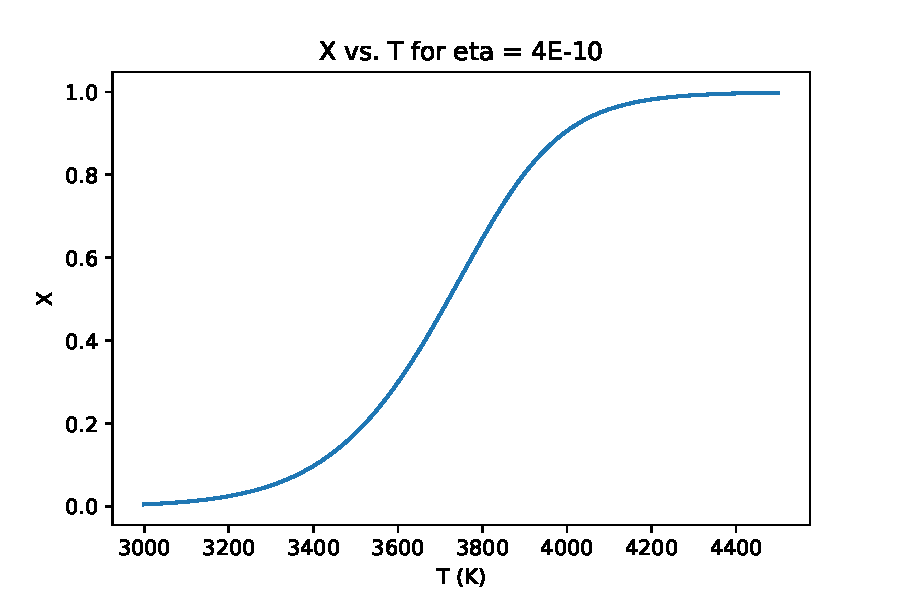
\includegraphics[scale=0.52]{Images/Q8-1eta4.pdf}
    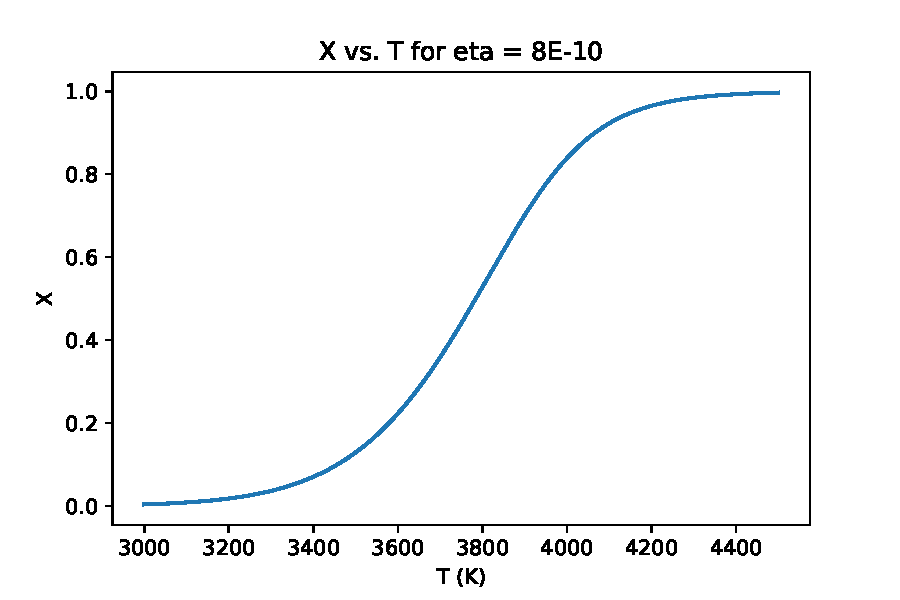
\includegraphics[scale=0.52]{Images/Q8-1eta8.pdf}
    
    \caption{Plots of fractional ionization $X$ as a function of temperature $T$ (in Kelvin) for baryon-to-photon ratios $\eta = 4 \times 10^{-10}$ and $\eta = 8 \times 10^{-10}$.}
    \label{fig-Q81}
\end{figure}

Taking $T_{\text{rec}}$ to be when $X = 1/2$, for $\eta = 4 \times 10^{-10}$, we have $\boxed{T_{\text{rec}} = 3720\si{K}}$, and for $\eta = 8 \times 10^{-10}$, we have $\boxed{T_{\text{rec}} = 3784\si{K}}$. Doubling the photon-to-baryon ratio has a small effect (only a relative change of about $1.7\%$).

\subsection{An ionizing photon per baryon}
From Problem 2.5, we recall:
\begin{equation}
    \frac{n(hf > E_0)}{n_\gamma} \approx 0.42\left(\frac{E_0}{kT}\right)^2\exp(-\frac{E_0}{kT})
\end{equation}
So setting $n(hf > E_0) = n_{\text{bary}}$ to have 1 ionizing photon per baryon, and letting $E_0 = Q$, we find:
\begin{equation}
    \eta = \frac{n_{\text{bary}}}{n_{\gamma}} = \frac{n(hf > Q)}{n_\gamma} = 0.42\left(\frac{Q}{kT}\right)^2\exp(-\frac{Q}{kT})
\end{equation}
With $Q = 13.6\si{eV}$ and $\eta = 6.1 \times 10^{-10}$, we can numerically solve the above relation to find:
\begin{equation}
    \boxed{T = 5823\si{K}}
\end{equation}
which is larger than the recombination temperature.

\subsection{}
(To be appended after HW is due)

\subsection{Distances to Last Scattering}
From Fig 5.9, we can see that at $z_{\text{ls}} = 1090$, the propert distance approaches its limiting value of $3.20c/H_0$, so:
\begin{equation}
    \boxed{d_{\text{p, ls}} = 3.20\frac{c}{H_0} = 14000\si{Mpc}}.
\end{equation}
Finding the luminosity distance is then just multiplying the above by a factor of $(1 + z_{\text{ls}})$:
\begin{equation}
    \boxed{d_{\text{L, ls}} = (1 + z_{\text{ls}})d_{\text{p, ls}} = 1091d_{\text{p, ls}} = 15274\si{Gpc}}.
\end{equation}
\newpage
\section[Nucleosynthesis and the Early Universe]{\hyperlink{toc}{Nucleosynthesis and the Early Universe}}

\subsection{Mass fraction of Helium with faster decay}
After the proton/neutron freezeout, the ratio of neutrons to protons is approximately:
\begin{equation}
    f_0 = \frac{n_{n, 0}}{n_{p, 0}} \approx \frac{1}{5}
\end{equation}
Suppose the time delay until nucleosynthesis is $t$. In this time delay, the neutrons decay to $\exp(-t/\tau_n)$ of their original amount, and the protons increase by the amount the neutrons decay (as the neutrons decay into a proton and electron). Therefore, the neutron-to-proton to ratio as a function of delay time is:
\begin{equation}\label{ntop}
    f(t) = \frac{n_n(t)}{n_p(t)} = \frac{n_{n, 0}\exp(-t/\tau_n)}{n_{p, 0} + n_{n, 0}(1 - \exp(-t/\tau_n))} = \frac{\frac{n_{n, 0}}{n_{p, 0}}\exp(-t/\tau_n)}{1 + \frac{n_{n, 0}}{n_{p, 0}}(1 - \exp(-t/\tau_n))} = \frac{f_0\exp(-t/\tau_n)}{1 + f_0(1 - \exp(-t/\tau_n))}
\end{equation}
The time delay from freezeout until nucleosynthesis is $200\si{s}$, and we suppose that the neutron decay time is reduced to $\tau_n = 88\si{s}$, so we can compute the fraction $f(200)$ at the time of nucleosynthesis to be:
\begin{equation}
    f(200) = 0.017
\end{equation}
If we assume that all available neutrons are incorporated into Helium, we get the maximal value for the primordial Helium fraction (as derived in problem 9.4) so:
\begin{equation}
    \boxed{Y_{\text{max}} = \frac{2f(200)}{1+f(200)} = 0.033}
\end{equation}

\subsection{Mass fraction of Helium with different rest energies}
Note that technically, this new difference in the mass fraction would likely cause some difference in the binding energy of the deuteron. This would affect the temperature $T_{\text{nuc}}$ of nucleosynthesis, as:
\begin{equation}
    1 \approx 6.5\eta\left(\frac{kT_{\text{nuc}}}{m_n c^2}\right)^{3/2}\exp(\frac{B_{D}}{kT_{\text{nuc}}})
\end{equation}
and therefore the nucleosynthsis time $t_{\text{nuc}}$ would also change. For simplicity's sake, let us assume that $B_D$ remains unchanged. However, the difference in the mass energy \emph{will} affect the neutron-to-proton ratio at freezeout, where we find:
\begin{equation}
    f_0 = \frac{n_{n, 0}}{n_{p, 0}} = \exp(-\frac{Q_{n}}{kT_{\text{freeze}}})
\end{equation}
so with $Q_{n} = 0.129\si{MeV}$ instead of $1.29\si{MeV}$ and $kT_{\text{freeze}} = 0.8\si{MeV}$, we find:
\begin{equation}
    f_0 = 0.85.
\end{equation}
So, using \eqref{ntop} with $f_0 = 0.85$, $t = 200\si{s}$, $\tau_n = 880\si{s}$, we find:
\begin{equation}
    f(200) = 0.58
\end{equation}
therefore the maximum possible mass fraction is given by:
\begin{equation}
    \boxed{Y_{\text{max}} = \frac{2f(200)}{1 + f(200)} = 0.734}
\end{equation}


\subsection{}
(To be appended after HW is due)

\subsection{Maximum value for primordial Helium Fraction}
By definition, we have:
\begin{equation}\label{Ymaxdef}
    Y_{\text{max}} = \frac{\rho_{\text{He}}}{\rho_{\text{b}}}
\end{equation}
Further, assuming that all neutrons are contained in Helium (as we want the maximal primordial Helium fraction), we have:
\begin{equation}
    \rho_{\text{He}} = 2\rho_{n}
\end{equation}
And the Baryonic density is given by:
\begin{equation}
    \rho_b = \rho_n + \rho_p
\end{equation}
Where:
\begin{equation}
    \rho_n = m_nn_n, \quad \rho_p = m_pn_p
\end{equation}
So substituting these into \eqref{Ymaxdef} we have:
\begin{equation}
    Y_{\text{max}} = \frac{2\rho_n}{\rho_n + \rho_p} = \frac{2\rho_n/\rho_p}{1 + \rho_n/\rho_p} = \frac{2\frac{n_n}{n_p}\frac{m_n}{m_p}}{1 + \frac{n_n}{n_p}\frac{m_n}{m_p}}
\end{equation}
Defining $f = \frac{n_n}{n_p}$ and making the approximation that $\frac{m_n}{m_p} \approx 1$, we conclude:
\begin{equation}
    \boxed{Y_{\text{max}} \approx \frac{2f}{1 + f}}
\end{equation}

\subsection{Neutrino Detection}
The cross-section for the interaction of a neutrino with a proton or neutron is:
\begin{equation}
    \sigma_w \sim 10^{-47}\si{m^2}\left(\frac{kT}{1\si{MeV}}\right)^2.
\end{equation}
So for a typical CNB neutrino with $E_\nu \sim kT_\nu \sim 5 \times 10^{-4}\si{eV}$, we have:
\begin{equation}
    \boxed{\sigma_w \sim 2.5 \times 10^{-66}\si{m^2}}
\end{equation}
Fe-56 has 26 protons, 26 electrons, and 30 neutrons per atom. It has a per-atom weight of:
\begin{equation}
    M = 26m_p + 26m_e + 30m_n \approx 56m_p = 56 \times 1.67 \times 10^{-27}\si{kg} =  9.34 \times 10^{-26}\si{kg}
\end{equation}
So the atomic number density is:
\begin{equation}
    n_a = \frac{\rho}{M} = \frac{7900\si{kg.m^{-3}}}{9.34 \times 10^{-26}\si{kg}} = 8.5 \times 10^{28}\si{m^{-3}}
\end{equation}
The number density of protons/electrons is therefore:
\begin{equation}
    \boxed{n_p = n_e = 26n_a = 2.2 \times 10^{30}\si{m^{-3}}}
\end{equation}
and the number density of neutrons is therefore:
\begin{equation}
    \boxed{n_n = 30n_a = 2.5 \times 10^{30}\si{m^{-3}}}
\end{equation}
The total number density of sub-atomic particles is therefore:
\begin{equation}
    n \sim n_p + n_e + n_n = 6.9 \times 10^{30}\si{m^{-3}}
\end{equation}
though of course this is approximate; really all the subatomic particles are clustered in their respective atoms. The mean free path of a CNB neutrino in this medium is given by:
\begin{equation}
    \boxed{\lambda = \frac{1}{n\sigma_w} = 5.8 \times 10^{34}\si{m}}
\end{equation}
\emph{Extremely} large; neutrinos are very hard to detect!

\subsection*{Optical Depth of Reionized Material (9.5 in first ed.)}
\addcontentsline{toc}{subsection}{\protect\numberline{}Optical Depth of Reionized Material (9.5 in first ed.)}
\begin{tcolorbox}
    We know from ovbservations that the intergalatic medium is currently ionized. Thus, at some point between $t_{\text{rec}}$ and $t_0$, the integalactic medium must have been reionized. In fact detailed measurements of the CMB on large scales place constraints on the amount of reionization (but that isn't important for this question). Assume that the baryonic component of the Universe instantaneously became completely reionized at some time $t_*$. For what value of $t_*$ does the optical depth of the reionized material:
    \begin{equation}
        \tau = \int_{t_*}^{t_0}\Gamma(t)\mathrm d t = \int_{t_*}^{t_0} n_e(t)\sigma_e c \mathrm d t
    \end{equation}
    equal one? For simplicity, assume that the Universe is spatially flat and matter-dominated, and that the baryonic component of the universe is pure hydrogen. To what redshift $z_*$ does this alue of $t_*$ correspond?
\end{tcolorbox}
\noindent
As the baryon density scales as $\propto \frac{1}{a^3}$, we have that:
\begin{equation}
    n_{e}(t)\sigma_e c = \frac{n_{e, 0}\sigma_e c}{a^3}
\end{equation}
Assuming that the baryonic component of the universe is pure hydrogen and that the universe is charge neutral, we have:
\begin{equation}
    n_{e, 0} = n_{\text{bary}, 0}
\end{equation}
For a flat, matter-dominated universe, we have scale factor (Ryden 5.5):
\begin{equation}
    a(t) = \left(\frac{t}{t_0}\right)^{2/3}
\end{equation}
so we find:
\begin{equation}
    n_{e}(t)\sigma_e c = \frac{n_{\text{bary}, 0}\sigma_e c t_0^2}{t^2}
\end{equation}
so carrying out the integral we have:
\begin{equation}
    1 = \tau = \int_{t_0}^{t_*}\frac{n_{\text{bary}, 0}\sigma_e c t_0^2}{t^2} \mathrm d t = n_{\text{bary}, 0}\sigma_e c t_0^2\left(\frac{1}{t_0} - \frac{1}{t_*}\right)
\end{equation}
So rearranging for $t_*$ we have:
\begin{equation}
    t_* = \frac{1}{\frac{1}{t_0} - \frac{1}{n_{\text{bary}, 0}\sigma_ec t_0^2}}
\end{equation}
In a flat, matter-dominated universe, the age of the universe is given by:
\begin{equation}
    t_0 = \frac{2}{3H_0}
\end{equation}
so we obtain:
\begin{equation}
    t_* = \frac{1}{\frac{3H_0}{2} - \frac{9H_0^2}{4n_{\text{bary}, 0}\sigma_ec}}
\end{equation}
Therefore, taking $H_0 = 68 \si{km.s^{-1}.Mpc^{-1}}$, $n_{\text{bary}, 0} = 0.25\si{m^{-3}}$, $c = 3 \times 10^{8}\si{m.s^{-1}}$, and $\sigma_e = 6.65 \times 10^{-29}\si{m^2}$, we find:
\begin{equation}
    \boxed{t_* = 4.2 \times 10^{14}\si{s} = 13 \si{Myr}}
\end{equation}
\newpage
\section[Inflation and the Very Early Universe]{\hyperlink{toc}{Inflation and the Very Early Universe}}

\subsection{Upper limit on Primordial Density}
Taking the hint, prior to inflation the Friedmann equation is dominated by the radiation and curvature term, so:
\begin{equation}
    \frac{H^2}{H_0^2} = \frac{\Omega_{r, 0}}{a^4} + \frac{1 - \Omega_{r, 0}}{a^2}
\end{equation}
Or writing $H = \frac{\dot{a}}{a}$:
\begin{equation}
    \frac{\dot{a}^2}{H_0^2} = \frac{\Omega_{r, 0}}{a^2} + 1 - \Omega_{r, 0}
\end{equation}
We take our reference time to be at $t = t_p$, so $H_0 = H_p$ and $\Omega_{r, 0} = \Omega(t_p)$ and hence:
\begin{equation}
    \frac{\dot{a}^2}{H_p^2} = \frac{\Omega(t_p)}{a^2} + 1 - \Omega(t_p)
\end{equation}
We can write $\dot{a} = \od{a}{t}$ and integrate both sides to obtain:
\begin{equation}
    H_p\int_{0}^{t} \mathrm d t = \int_{0}^{a}\frac{a'\mathrm d a}{\sqrt{\Omega(t_p) + (1 - \Omega(t_p))a'^2}}
\end{equation}
Where we set $a(t = 0) = 0$. In order to perform the integral on the LHS, we make the substitution $u = \Omega(t_p) + (1 - \Omega(t_p))a'^2$ which gives $du = 2(1 - \Omega(t_p))a' da'$. It also changes the bouds of integration to be from $\Omega(t_p)$ to $\Omega(t_p) + (1 - \Omega(t_p))a^2$. We therefore obtain:
\begin{equation}
    H_p t = \int_{\Omega(t_p)}^{\Omega(t_p) + (1 - \Omega(t_p))a^2} \frac{1}{2(1 - \Omega(t_p))}\frac{1}{\sqrt{u}}\mathrm d u
\end{equation}
This integral can now be performed to obtain:
\begin{equation}
    H_p t = \frac{1}{2(1 - \Omega(t_p))} \left(\left. 2\sqrt{u}\right|_{\Omega(t_p)}^{\Omega(t_p) + (1 - \Omega(t_p))a^2}\right) = \frac{1}{1 - \Omega(t_p)}\left(\sqrt{\Omega(t_p) + (1 - \Omega(t_p))a^2}- \sqrt{\Omega(t_p)}\right)
\end{equation}
We can now solve for $a(t)$:
\begin{equation}
    a(t) = \sqrt{\frac{\left[(1 - \Omega(t_p))H_p t +  \sqrt{\Omega(t_p)} \right]^2 - \Omega(t_p)}{(1 - \Omega(t_p))}}
\end{equation}
In order to find a maximum permissable value of $\Omega(t_p)$, we want to see the big crunch exactly at the start of the inflationary epoch at $t_i$, so:
\begin{equation}
    a(t_i) =  \sqrt{\frac{\left[(1 - \Omega(t_p))H_p t_i +  \sqrt{\Omega(t_p)} \right]^2 - \Omega(t_p)}{(1 - \Omega(t_p))}} = 0
\end{equation}
From this we obtain:
\begin{equation}
    (1 - \Omega(t_p))H_p t_i +  \sqrt{\Omega(t_p)}= \pm \sqrt{\Omega(t_p)}
\end{equation}
If $t_i = 0$ we have that the LHS equals $+ \sqrt{\Omega(t_p)}$, but since we want $t_i > 0$, we solve for the negative solution. this yields:
\begin{equation}
    H_pt_i = \frac{-2\sqrt{\Omega(t_p)}}{1 - \Omega(t_p)}
\end{equation}
From the previous question, we know that $H = \frac{1}{2t}$ in a radiation-dominated universe, so $H_p = \frac{1}{2t_p}$ and so:
\begin{equation}
    \frac{t_i}{2t_p} = \frac{2\sqrt{\Omega(t_p)}}{\Omega(t_p) - 1}
\end{equation}
For conveninece, let us define $\alpha = \frac{t_i}{4t_p}$:
\begin{equation}
    \alpha = \frac{\sqrt{\Omega(t_p)}}{\Omega(t_p) - 1}
\end{equation}
Rearranging, we find a quadratic equation in $\Omega(t_p)$:
\begin{equation}
    \Omega(t_p)^2 - (2 + \frac{16 t_p^2}{t_i^2})\Omega(t_p) + 1 = 0
\end{equation}
This has solutions:
\begin{equation}
    \Omega(t_p) = \frac{(2 + \frac{16 t_p^2}{t_i^2}) \pm \sqrt{(2 + \frac{16 t_p^2}{t_i^2})^2 - 4}}{2}
\end{equation}
Since $\Omega(t_p) > 1$, we reject the negative solution above. So, the maximum possible $\Omega(t_p)$ is given by:
\begin{equation}
    \boxed{\Omega(t_p) = \frac{(2 + \frac{16 t_p^2}{t_i^2}) +  \sqrt{\frac{64 t_p^2}{t_i^2} + \frac{256 t_p^4}{t_i^4}}}{2}}
\end{equation}
Since $t_p \ll t_i$, we can neglect all powers of $\frac{t_p}{t_i}$ in the above expression that are higher than linear order. This yields:
\begin{equation}
    \boxed{\Omega(t_p) \approx 1 + 4\frac{t_p}{t_i}}
\end{equation}
For $t_i = 10^{-36}\si{s}$, we have:
\begin{equation}
    \boxed{\Omega(t_p) = 1 + 2 \times 10^{-7}}
\end{equation}
For $t_i = 10^{-26}\si{s}$, we have:
\begin{equation}
    \boxed{\Omega(t_p) = 1 + 2 \times 10^{-17}}
\end{equation}

\subsection{Solving the Monopole Problem}
If monopoles formed at the GUT time with one monopole per horizon of mass $m_M = m_{GUT}$, then the energy density of these monopoles would be given by:
\begin{equation}
    e_M(t_{GUT}) \approx \frac{m_Mc^2}{(2ct_{GUT})} = 10^{106}\si{eV.m^{-3}}
\end{equation}
where we take $m_Mc^2 \sim E_{GUT} \sim 10^{12}\si{TeV}$ and $t_{GUT} = 10^{-36}\si{s}$. Therefore the density parameter of the monopoles at this time is given by:
\begin{equation}
    \Omega_M(t_{GUT}) = \frac{\e_{M}(t_{GUT})}{\e_{c, 0}} \approx 10^{96}
\end{equation}
where we take $\e_{c, 0} = 5 \times 10^9\si{eV.m^{-3}}$. For a radiation-only universe, the scale factor goes as (Ryden Eq. 5.60):
\begin{equation}
    a(t) = \left(\frac{t}{t_0}\right)^{1/2}
\end{equation}
So at the GUT time:
\begin{equation}
    a(t_{GUT}) = \left(\frac{t_{GUT}}{t_0}\right)^{1/2}
\end{equation}
Taking $t_0 \sim 13.8\si{Gyr} = 4.35 \times 10^{17}\si{s}$ and $t_{GUT}$ as before, we find:
\begin{equation}
    a(t_{GUT}) = 1.5 \times 10^{-27}.
\end{equation}
Since the magnetic monopole density parameter should scale as $\frac{1}{a^3}$ with time (like regular matter), if inflation did not happen, the density of monopoles today would be:
\begin{equation}
    \Omega_M(t_0) = \Omega_M(t_{GUT})a(t_{GUT})^3 = 3.4 \times 10^{15}
\end{equation}
This is off from the observational limits by:
\begin{equation}
    \frac{\Omega_{M, 0, \text{observed}}}{\Omega_M(t_0)} = \frac{10^{-6}}{3.4 \times 10^{15}} = 2.9 \times 10^{-22}.
\end{equation}
To account for this, we must have had $N$ e-folds of inflation, leading the scale factor is actually $e^{N}$ larger than what we calculated above. Hence:
\begin{equation}
    2.9 \times 10^{-22} = \frac{1}{e^{3N}}
\end{equation}
which we can solve for $N$ to obtain:
\begin{equation}
    \boxed{N \approx 17}
\end{equation}


\subsection{False Vacuum}
The Universe dominated by the false vacuum has the same structure as one with dominated by a cosmological constant. In such a universe, the Hubble parameter s given by Ryden 5.72:
\begin{equation}
    \boxed{H_i = \left(\frac{8\pi G\e_{\Lambda}}{3c^2}\right)^{1/2} = 1.83 \times 10^{-18}\si{s^{-1}} = 0.83H_0}
\end{equation}
where we take $H_0$ is the Hubble constant in our universe. We assume that at the false vacuum decay time that the false vacuum decays into blackbody photons, so we can therefore use the blackbody radiation temperature to solve for what the temperature of the Universe would be at this time:
\begin{equation}
    \boxed{T = \sqrt[4]{\frac{\e_{\Lambda}}{\alpha}} = 29\si{K}}
\end{equation}
To find the energy density of matter at this time, we first compute the scale factor at this time; this is given by Ryden 5.73 to be:
\begin{equation}
    a(t_f) = a(t_0)e^{H_i(t_f - t_0)} = e^{H_i(t_f - t_0)} 
\end{equation}
where we take $a(t_0) = 1$ by convention. So with $H_i$ as above, $t_f = 50t_0$ and $t_0 = 13.7\si{Gyr}$, we find:
\begin{equation}
    a(t_f) = 6.7 \times 10^{16}
\end{equation}
So the energy density of matter at this time would be:
\begin{equation}
    \boxed{\e_{m}(t_f) = a(t_f)^{-3} \e_{m, 0} = 5 \times 10^{-48}\si{MeV.m^{-3}}}
\end{equation}
To find when the universe is again dominated by matter, we wish to find the time when:
\begin{equation}\label{matterradequality}
    \e_{m} = \e_r.
\end{equation}
Further, we know that:
\begin{equation}\label{matterradscaling}
    \e_m(a) = \frac{\e_{m, 0}}{a^3}, \quad \e_{r}(a) = \frac{\e_{r, 0}}{a^4}
\end{equation}
First solving for what $\e_{r, 0}$ would be, we have:
\begin{equation}
    \e_{r, 0} = \e_{r}(t_f)a(t_f)^4 = 6.7 \times 10^{70}\si{MeV.m^{-3}}
\end{equation}
Combining \eqref{matterradequality} and \eqref{matterradscaling} we find:
\begin{equation}
    \frac{\e_{m, 0}}{a_{rm}^3} = \frac{\e_{r, 0}}{a_{rm}^4}
\end{equation}
Hence:
\begin{equation}
    a_{rm} = \frac{\e_{r, 0}}{\e_{m, 0}}
\end{equation}
Further in a radiation dominated universe we know we have $a(t) = \left(\frac{t}{t_0}\right)^{1/2}$ (Ryden Eq. 5.60), so:
\begin{equation}
    \boxed{t_{rm} = t_0 \left(\frac{\e_{r, 0}}{\e_{m, 0}}\right)^2}
\end{equation}
Numerically we obtain:
\begin{equation}
    \boxed{t_{rm} = 2.7 \times 10^{136}\si{Gyr}}
\end{equation}

\subsection*{Gamow's CMB Prediction (10.3 in first ed.)}
\addcontentsline{toc}{subsection}{\protect\numberline{}Gamow's CMB Prediction (10.3 in first ed.)}
\begin{tcolorbox}
    A fascinating bit of cosmological history is that of George Gamow's prediction of the Cosmic Microwave Background in 1948. (Unfortunately, his prediction was premature; by the time the CMB was actually discovered in the 1960's, his prediction had fallen into obscurity.) Let's see if you can reproduce Gamow's line of argument. Gamow knew that nucleosynthesis must have taken place at a temperature $T_{\text {nuc }} \simeq 10^{9} \mathrm{~K}$, and that the age of the Universe is currently $t_{0} \simeq 10 \mathrm{Gyr}$. Assume that the Universe is flat and contains only radiation. With these assumptions, what was the energy density $\epsilon$ at the time of nucleosynthesis? What was the Hubble parameter $\mathrm{H}$ at the time of nucleosynthesis? What was the time $t_{\text {nuc }}$ at which nucleosynthesis took place? What is the current temperature $T_{0}$ of the radiation filling the Universe today? If the Universe switched from being radiation-dominated to being matter-dominated at a redshift $z_{r m}>0$, will this increase or decrease $T_{0}$ for fixed values of $T_{\text {nuc }}$ and $t_{0}$ ? Explain your answer.
\end{tcolorbox}
\noindent 
If the Universe only contains radiation, the energy density is given by the black body energy density formula:
\begin{equation}
    \e_\gamma(T) = \alpha T^4
\end{equation}
So with $\alpha = 7.566\times 10^{-16}\si{J.m^{-3}.K^{-4}}$ and $T_{\text{nuc}} = 10^{9}\si{K}$ we have:
\begin{equation}
    \boxed{\e_{\text{nuc}} = \alpha T_{\text{nuc}}^4 = 7.566 \times 10^{20} \si{J.m^{-3}}}
\end{equation}
Furthermore, Ryden Eq. 5.63 gives the energy density in a radiation-only universe as a function of time to be:
\begin{equation}
    \e(t) = 0.030\frac{E_p}{l_p^3}\left(\frac{t}{t_p}\right)^{-2}
\end{equation}
We can invert the above formula to find $t_{\text{nuc}}$:
\begin{equation}
    t_{\text{nuc}} = \sqrt{0.030\frac{E_p}{l_p^3}}\frac{t_p}{\sqrt{\e(t_{\text{nuc}})}}
\end{equation}
which numerically gives:
\begin{equation}
    \boxed{t_{\text{nuc}} = 230\si{s}}
\end{equation}
Next, in a radiation dominated universe, we have (from Ryden Eq. 5.60):
\begin{equation}
    a(t) = \left(\frac{t}{t_0}\right)^{1/2}
\end{equation}
So the Hubble parameter is given by:
\begin{equation}
    H = \frac{\dot{a}}{a} = \frac{1}{2t}
\end{equation}
So at nucleosynthesis:
\begin{equation}
    \boxed{H_{\text{nuc}} = 4.3 \times 10^{-3}\si{s^{-1}}}
\end{equation}
The energy density of radiation scales as $\frac{1}{a^4}$, so we can use this to find the energy density of the universe today:
\begin{equation}
    \e_{r, 0} = \e_{\text{nuc}}a_{\text{nuc}}^4 = \e_{\text{nuc}}\left(\frac{t_{\text{nuc}}}{t_0}\right)^{2}
\end{equation}
so we can find the current temperature (which is still described by a black body) as:
\begin{equation}
    \alpha T_0^4 = \alpha T_{\text{nuc}}^4\left(\frac{t_{\text{nuc}}}{t_0}\right)^{2}
\end{equation}
\begin{equation}
    T_0 =  T_{\text{nuc}}\left(\frac{t_{\text{nuc}}}{t_0}\right)^{1/2}
\end{equation}
Numerically we find:
\begin{equation}
    \boxed{T_0 = 27\si{K}}
\end{equation}
Now, we suppose that the Universe switched from being radiation-dominated to matter-dominated at some redshift $z_{rm} > 0$. This would not change the energy density at the time of nucleosynthesis, but the scale factor would now grow as:
\begin{equation}
    a(t) = \left(\frac{t}{t_0}\right)^{2/3}
\end{equation}
instead of the previous $\propto t^{1/2}$. Hence the energy density of the radiation would go down more rapidly than in the radiation-dominated-for-all times Universe, and hence the temperature $T_0$ today would $\boxed{\text{decrease}}$.
\newpage
\section[Structure Formation: Gravitational Instability]{\hyperlink{toc}{Structure Formation: Gravitational Instability}}

\subsection{Density Fluctuations in a Flat, Matter-Dominated, Contracting Universe}
We first note that:
\begin{equation}
    H = \frac{\dot{a}}{a} < 0
\end{equation}
in a contracting universe. Now, starting with Ryden Eq. 11.49, we have:
\begin{equation}
    \ddot{\delta} + 2H\dot{\delta} - \frac{3}{2}\Omega_m H^2\delta = 0
\end{equation}
In a contracting matter dominated universe, $\Omega_m = 1$ and $H = -\frac{2}{3t}$ (note the negative sign for contraction! This can be obtained from $a(t) = \left(\frac{t}{t_0}\right)^{2/3}$), so:
\begin{equation}
    \ddot{\delta} - \frac{4}{3t}\dot{\delta} - \frac{2}{3t^2}\delta = 0
\end{equation}
Guessing a power law $\delta(t) = t^r$, we find:
\begin{equation}
    r(r-1)t^{r-2} - \frac{4}{3t}rt^{r-1} - \frac{2}{3t^2}t^r = 0
\end{equation}
Dividing both sides by $t^{r-2}$ we obtain a quadratic equation for $r$:
\begin{equation}
    r^2 - \frac{7}{3}r - \frac{2}{3} = 0
\end{equation}
Using the quadratic formula, we find the solutions:
\begin{equation}
    r = \frac{7 \pm \sqrt{73}}{6}
\end{equation}
So we therefore find:
\begin{equation}
    \boxed{\delta(t) = At^{\frac{7 + \sqrt{73}}{6}} + Bt^{\frac{7 - \sqrt{73}}{6}}}
\end{equation}
Where $A, B$ are constants determined by initial conditions. The second term vanishes for large $t$, so:
\begin{equation}
    \boxed{\delta(t) \approx At^{\frac{7 + \sqrt{73}}{6}}}
\end{equation}

\subsection{Density Fluctuations in a Nearly Empty, Negatively Curved, Expanding Universe}
We again start with Ryden Eq. 11.49:
\begin{equation}
    \ddot{\delta} + 2H\dot{\delta} - \frac{3}{2}\Omega_m H^2\delta = 0
\end{equation}
Since $\Omega_m \ll 1$, the last term can be neglected:
\begin{equation}
    \ddot{\delta} + 2H\dot{\delta} = 0
\end{equation}
In an empty expanding universe, we have $H = \frac{1}{t}$ (as $a(t) = \frac{t}{t_0}$) so:
\begin{equation}
    \ddot{\delta} + \frac{2}{t}\dot{\delta} = 0
\end{equation}
Again guessing a power law $\delta(t) = t^r$, we find:
\begin{equation}
    r(r-1)t^{r-2} + \frac{2}{t}rt^{r-1} = 0
\end{equation}
Dividing both sides by $t^{r-2}$ we obtain a quadratic equation for $r$:
\begin{equation}
    r^2 + r = 0
\end{equation}
This has solutions:
\begin{equation}
    r = 0, r = -1
\end{equation}
So we therefore find:
\begin{equation}
    \boxed{\delta(t) = At^0 + Bt^{-1}}
\end{equation}
At long times, the latter terms vanishes, so:
\begin{equation}
    \boxed{\delta(t) \approx A}.
\end{equation}
That is, at long times the fluctuations are constant.

\subsection{Photon-Baryon Fluid (ADD LATER)}
\subsection{Galaxy Formation by Gravitational Collapse (ADD LATER)}

\subsection{}

\subsection{Mean Square Mass Fluctuation and Standard Deviation of Density Field}
The standard deviation of the density field for a Gaussian field can be computed (in the case of a Gaussian field) as (Ryden Eq. 11.67):
\begin{equation}
    \sigma_\delta^2 = \frac{V}{2\pi}\int_0^\infty P(k)k^2 \mathrm dk = \frac{V}{2\pi}\int_0^{k_{max}} P(k)k^2 \mathrm dk
\end{equation}
Meanwhile the mean square mass fluctuation is computed as:
\begin{equation}
    \avg{\left(\frac{\delta M}{M}\right)^2} = \avg{\left(\frac{M  - \avg{M}}{\avg{M}}\right)^2} = \frac{V}{2\pi }\int_0^{\infty}P(k)\left[\frac{3j_1(kr)}{kr}\right]^2 k^2 \mathrm d k = \frac{V}{2\pi }\int_0^{k_{\text{max}}}P(k)\left[\frac{3j_1(kr)}{kr}\right]^2 k^2 \mathrm d k 
\end{equation}
So the claim is proven is we can show for $M < M_{\text{min}}$, or for $r < r_{\text{min}}$ that:
\begin{equation}
    \int_{0}^{k_{max}} P(k)k^2 \mathrm d k = \int_0^{k_{\text{max}}}P(k)\left[\frac{3j_1(kr)}{kr}\right]^2 k^2 \mathrm d k 
\end{equation}
Incoming is a handwavey argument that I don't actually think is the full answer. For $r < r_{\text{min}} = \frac{2\pi}{k_{\text{max}}}$, $kr$ will be small over the domain of integration so we may Taylor expand $j_1(kr)$. Doing so, we find:
\begin{equation}
    j_1(kr) = \frac{\sin(kr) - kr\cos(kr)}{(kr)^2} \approx \frac{(kr - \frac{(kr)^3}{6}) - kr\left(1 - \frac{(kr)^2}{2}\right)}{(kr)^2} = \frac{\frac{(kr)^3}{3}}{(kr)^2} = \frac{kr}{3}
\end{equation}
Therefore:
\begin{equation}
    \int_0^{k_{\text{max}}}P(k)\left[\frac{3j_1(kr)}{kr}\right]^2 k^2 \mathrm d k \approx  \int_0^{k_{\text{max}}}P(k)\left[\frac{3}{kr}\frac{kr}{3}\right]^2 k^2 \mathrm d k = \int_0^{k_{\text{max}}}P(k) k^2 \mathrm d k
\end{equation}
Which is exactly what we wished to show.
\newpage
\section[Structure Formation: Baryons and Photons]{\hyperlink{toc}{Structure Formation: Baryons and Photons}}

\subsection{Galaxies more luminous than $L$}
We start with the Schechter luminosity function which gives the number density $\Phi(L)\mathrm d L$ in the range $L \rightarrow L + \mathrm d L$:
\begin{equation}
    \Phi(L) \mathrm d L = \Phi^*\left(\frac{L}{L^*}\right)^\alpha\exp(-\frac{L}{L^*})\frac{\mathrm d L}{L^*}
\end{equation}
The number density of galaxies more luminous than $L$ is given by integrating from $L$ to $\infty$:
\begin{equation}
    n_{\geq L} = \int_L^\infty \Phi(L')\mathrm d L' = \int_L^\infty \Phi^*\left(\frac{L'}{L^*}\right)^\alpha\exp(-\frac{L'}{L^*})\frac{\mathrm d L'}{L^*}
\end{equation}
Now substituting $t = \frac{L'}{L^*}$ which gives $\mathrm d t = \frac{\mathrm d L'}{L^*}$ we find:
\begin{equation}
    n_{\geq L} = \Phi^* \int_{L/L^*}^\infty t^\alpha e^{-t} \mathrm d t
\end{equation}
Furthermore, we can recognize the RHS as an incomplete gamma function, yielding:
\begin{equation}
    \boxed{n_{\geq L} = \Phi^* \Gamma(\alpha + 1, \frac{L}{L^*})}
\end{equation}
In the limit $L \to 0$, we just have the regular gamma function:
\begin{equation}
    n_{\geq 0} = n_{\text{tot}} = \Phi^* \int_0^\infty t^\alpha e^{-t}\mathrm d t = \Phi^*\Gamma(\alpha + 1)
\end{equation}
But with $\alpha = -1$, the integral:
\begin{equation}
    n_{\text{tot}} =\int_0^\infty \frac{e^{-t}}{t}\mathrm d t = \infty
\end{equation}
is seen to diverge (at the lower limit). The physical solution is as follows; in this limit, the number density of galaxies diverges, but the luminosity density remains finite (so the average luminosity per galaxy is zero); this can be realized via the following calculation:
\begin{equation}
    \Psi_{\text{tot}} = \int_0^\infty L'\Phi(L')\mathrm d L = \int_0^\infty L'\Phi^*\left(\frac{L'}{L^*}\right)^{-1}\exp(-\frac{L'}{L^*})\frac{\mathrm d L'}{L^*} = 
    \Phi^*\int_0^\infty \exp(-\frac{L'}{L^*})\mathrm d L' = \Phi^*L^*.
\end{equation}

\subsection{Total Luminosity Density}
We again tart with the Schechter luminosity function:
\begin{equation}
    \Phi(L) \mathrm d L = \Phi^*\left(\frac{L}{L^*}\right)^\alpha\exp(-\frac{L}{L^*})\frac{\mathrm d L}{L^*}
\end{equation}
We can now integrate $L \Phi(L)\mathrm d L$ from $0$ to $\infty$ to obtain the total luminosity density:
\begin{equation}
    \Psi = \int_0^\infty \Phi(L') \mathrm d L' = \int_0^\infty L'\Phi^*\left(\frac{L'}{L^*}\right)^{\alpha}\exp(-\frac{L'}{L^*})\frac{\mathrm d L'}{L^*} = \int_0^\infty \Phi^*\left(\frac{L'}{L^*}\right)^{\alpha+1}\exp(-\frac{L'}{L^*})\mathrm d L'
\end{equation}
Again making the substitution $t = \frac{L'}{L^*}$ we find:
\begin{equation}
    \Psi = \int_0^\infty \Phi^*L^* t^{\alpha+1} e^{-t}\mathrm d t = \Phi^*L^*\int_0^\infty t^{\alpha + 1}e^{-t}\mathrm d t
\end{equation}
We recognize the rightmost expression as a gamma function, which yields:
\begin{equation}
    \boxed{\Psi = \Phi^*L^*\Gamma(\alpha + 2)}
\end{equation}
Now, observing that $\Gamma(-1 + 2) = \Gamma(1) = 1$, so we find for the $V$ band that:
\begin{equation}
    \boxed{\Psi_V = \Phi^*L^*_V\Gamma(1) = 1 \times 10^8 \si{L_{\odot, V} Mpc^{-3}}}
\end{equation}

\subsection{Do structures of $10^{17}M_\odot$ exist today?}
From Ryden Eq. 12.38, the total amount of mass inside the last scattering surface is given by:
\begin{equation}
    M_{\text{tot}} \approx 4.3 \times 10^{23}M_\odot
\end{equation}
Dividing this by $M = 10^{17}M_\odot$, we find:
\begin{equation}
    N = \frac{M_{\text{tot}}}{M} = 4.3 \times 10^6 \si{regions}
\end{equation}
The very first $M = 10^{17}M_\odot$ structure to collapse is the one region out of 4.3 million that had the highest overdensity at the time of radiation-matter equality, with probability:
\begin{equation}
    P = \frac{1}{N} = 2.3 \times 10^{-7}.
\end{equation}
This is equivalent to a $5.04\sigma$ deviation in a Gaussian distribution. Since $\sigma = \delta M/M = 0.12$, then we can compute the redshift of collapse to be:
\begin{equation}
    1 + z_{\text{coll}} = 5.04\sigma = 0.6048
\end{equation}
i.e. the first such object has not begin to collapse (as $z_{\text{coll}} < 0$) and hence $\boxed{\text{we do not}}$ expect to see gravitationally collapsed structures with mass $M = 10^{17}M_\odot$ today.

\subsection{Ripping Apart Galaxies}
An object is ripped apart when its energy density $\e_m$ becomes less than the phantom energy density $\e_p$. Hence we can set these two densities to be equal:
\begin{equation}
    \e_m = \e_p.
\end{equation}
We know that $\e_p \propto a^{-3(1+w_p)}$, and in particular:
\begin{equation}
   \e_p = \Omega_{p, 0}\e_c a^{-3(1+w_p)}.
\end{equation}
So solving for the rip-apart scale factor $a$ we find:
\begin{equation}
    a = \left(\frac{\e_m}{\Omega_p \e_c}\right)^{-1/(3+3w_p)}
\end{equation}
and for $w_p = -1.1$ this becomes:
\begin{equation}
    a = \left(\frac{\e_m}{\Omega_p \e_c}\right)^{10/3}.
\end{equation}
For the milky way galaxy, we have $M_{\text{gal}} = 9.6 \times 10^{11}M_\odot$ and $R_{\text{gal}} = 75\si{kpc}$. Assuming a uniform mass density and using that $\rho_c = 8.7 \times 10^{-27}\si{kg.m^{-3}}$, we find:
\begin{equation}
    \frac{\e_\text{gal}}{\e_c} = \frac{\rho_{\text{gal}}}{\rho_c} = \frac{M_{\text{gal}}}{\frac{4}{3}\pi R_{\text{gal}}^3 \rho_c} = 4.2 \times 10^{3}
\end{equation}
Therefore the scale factor for which the Milky way galaxy would be ripped apart can be solved to be:
\begin{equation}
    \boxed{a_{\text{gal}} = 4.0 \times 10^{12}}
\end{equation} 
We can do the same for the sun, with mass $M_\odot$ and radius $R_\odot = 7 \times 10^8 \si{m}$ to find:
\begin{equation}
    \frac{\e_{\text{sun}}}{\e_c} = \frac{\rho_{\text{sun}}}{\rho_c} = \frac{M_\odot}{\frac{4}{3}\pi R_\odot^3 \rho_c} = 1.6 \times 10^{29}
\end{equation}
so the scale factor for which the sun would be ripped apart would be:
\begin{equation}
    \boxed{a_{\text{sun}} = 7.2 \times 10^{97}}
\end{equation}

From Problem 5.5, we know the time between the present time $t_0$ and the Big rip $t_{\text{rip}}$ was found for $H_0 = 68\si{km.s^{-1}.Mpc^{-1}}$, $w_p = -1.1$ and $\Omega_{m, 0} = 0.3$ to be:
\begin{equation}
    t_{\text{rip}} - t_0 = 115.5\si{Gyr}
\end{equation}
with $t_0 = 13.8 \si{Gyr}$, we can find $t_{\text{rip}}$ to be:
\begin{equation}
    t_{\text{rip}} = 115.5\si{Gyr} - 13.8\si{Gyr} = 101.7\si{Gyr}
\end{equation}
Further, we can use the intermediate result from problem 5.5 (Eq. \eqref{int55}) that:
\begin{equation}
    \int_{t_0}^{t_{\text{rip}}}H_0 dt  \approx \int_1^\infty a^{3(1+w_p)/2}(1 - \Omega_{m, 0})^{-1/2}\mathrm d a = \frac{1}{\sqrt{\Omega_{p, 0}}}\int_1^\infty a^{3(1+w_p)/2-1}\mathrm d a
\end{equation}
Now, we can replace $t_0$ with $t_{\text{gal}}$ (the rip-apart time for the Milky Way Galaxy), and $a(t_0) = 1$ with $a(t_{\text{gal}}) = a_\text{gal}$ in the above equation, and carry out the integral to get:
\begin{equation}
    H_0(t_{\text{rip}} - t_{\text{gal}}) = \frac{1}{\sqrt{\Omega_{p, 0}}}\left.\frac{2}{3(1+w_p)}a^{3(1+w_p)/2}\right|_{a_{\text{gal}}}^\infty
\end{equation}
The term at infinity vanishes (as the exponent of $a$ is negative), and we therefore find:
\begin{equation}
    t_{\text{gal}} = t_{\text{rip}} - \frac{1}{H_0\sqrt{\Omega_{p, 0}}}\frac{2}{3\abs{1 + w_p}}a_{\text{gal}}^{3(1+w_p)/2}
\end{equation}
Numerically, this evaluates to:
\begin{equation}
    \boxed{t_{\text{gal}} = 101.7\si{Gyr} - 0.46\si{Gyr} = 101.w\si{Gyr}}
\end{equation}
So we find that the Milky way will be ripped apart about half a gigayear before the big rip. We can do the same with $t_{\text{sun}}$ and $a(t_\text{sun}) = a_{\text{sun}}$ to find:
\begin{equation}
    \boxed{t_{\text{sun}} = 101.7\si{Gyr} - 7.5\times 10^{-14}\si{Gyr} \approx 101.7\si{Gyr}}
\end{equation}
In other words, the sun will not be ripped apart until the big rip.




\end{document}